\documentclass{article}

\usepackage[utf8]{inputenc}
\usepackage[T1]{fontenc}
\usepackage{amsmath,amssymb,amsthm}
\usepackage{stmaryrd}
\usepackage[table]{xcolor}
\usepackage{mathtools}
\usepackage{hyperref}
\usepackage{cleveref}
\usepackage{booktabs}
\usepackage{enumitem}
\usepackage{listings}
\usepackage{xcolor}
\usepackage[margin=1in]{geometry}
\usepackage{braket}
\usepackage{microtype}
\usepackage{authblk}
\usepackage{blkarray}
\usepackage{thmtools}
\usepackage{tikz-cd}
\usepackage{physics}
\usepackage[most]{tcolorbox}
%\usepackage{unicode-math}

\newtcolorbox{mybox}[1][]{
    breakable,                % This allows the box to split across pages
    colback=blue!5!white,      % Background color
    colframe=blue!75!black,    % Border and title bar color
    % fonttitle controls the style of the title text
    fonttitle=\bfseries\large,
    title={#1},       % Title text
    enhanced,                  % Allows for more styling
    attach boxed title to top left={yshift=-2mm, xshift=2mm},
    boxed title style={colback=blue!75!black},
    #1                         % Allows for additional local arguments
}

\DeclareMathOperator{\Fun}{Fun}


\lstdefinelanguage{Lean}{
  morekeywords={def,theorem,lemma,structure,where,abbrev,noncomputable,let,fun,if,then,else,by,sorry,import,variable,instance,section,end,open,set_option,example,class,inductive,namespace,match,with,do,return,have,show,calc,suffices,obtain,rcases,refine,exact,apply,intro,intros,rw,simp,unfold,dsimp,constructor,cases,induction},
  sensitive=true,
  morecomment=[l]{--},
  morecomment=[s]{/-}{-/},
  morestring=[b]",
  literate={:=}{$\coloneqq$}2
}

\lstset{
  language=Lean,
  basicstyle=\small\ttfamily,
  keywordstyle=\color{blue!70!black}\bfseries,
  commentstyle=\color{green!50!black}\itshape,
  stringstyle=\color{red!60!black},
  breaklines=true,
  frame=single,
  framerule=0.4pt,
  rulecolor=\color{gray!50},
  backgroundcolor=\color{gray!5},
  xleftmargin=2em,
  xrightmargin=1em,
  aboveskip=0.8em,
  belowskip=0.8em,
  columns=flexible,
  mathescape=true,
  keepspaces=true,
  showstringspaces=false,
  escapeinside={(*@}{@*)},
  extendedchars=true,
  literate={↥}{{$\uparrow$}}1
           {≤}{{$\le$}}1
           {≥}{{$\ge$}}1
           {→}{{$\to$}}1
           {ℕ}{{$\mathbb{N}$}}1
           {⊢}{{$\vdash$}}1
           {₁}{{$_1$}}1
           {₂}{{$_2$}}1
           {ₛₗ}{{$_{\text{sl}}$}}1
           {ℂ}{{$\mathbb{C}$}}1
           {∑}{{$\sum$}}1
           {‖}{{$||$}}1
           {ₙ}{{$_n$}}1
           {α}{{$\alpha$}}1
           {β}{{$\beta$}}1
           {γ}{{$\gamma$}}1
           {×}{{$\times$}}1
           {ψ}{{$\psi$}}1
           {⟨}{{$\langle$}}1
           {⟩}{{$\rangle$}}1
           {•}{{$\bullet$}}1
           {∈}{{$\in$}}1
           {∀}{{$\forall$}}1
           {←}{{$\leftarrow$}}1
           {₀}{{$_0$}}1
           {λ}{{$\lambda$}}1
           {↥}{{$\uparrow$}}1
           {↪}{{$\hookrightarrow$}}1
           {∧}{{$\wedge$}}1
           {≃}{{$\simeq$}}1
           {ₘ}{{$_m$}}1
           {∃}{{$\exists$}}1
           {⊗}{{$\otimes$}}1
           {ₚ}{{$_p$}}1
           {⁻¹}{{$^{-1}$}}1
           {∉}{{$\notin$}}1
           {⊆}{{$\subseteq$}}1
           {¬}{{$\neg$}}1
           {ₓ}{{$_x$}}1
}



\newcommand{\Draft}{}

\ifdefined\Draft
\newcommand{\Ethan}[1]{{\color{magenta} [Yi: #1]}}
\newcommand{\RT}[1]{{\color{red} [Runzhou: #1]}}
\newcommand{\ME}[1]{{\color{blue} [Mati: #1]}}

\else
\newcommand{\Ethan}[1]{}
\newcommand{\RT}[1]{}
\newcommand{ME}[1]{}
\fi

\newcommand{\bbN}{\mathbb{N}}
\newcommand{\bbU}{\mathbb{U}}
\newcommand{\bbP}{\mathbb{P}}
\newcommand{\PauliFold}{\mathsf{PauliFold}}
%\DeclareMathOperator{\PauliFold}{PauliFold}
\DeclareMathOperator{\Image}{Image}

\newtheorem{theorem}{Theorem}[section]
\newtheorem{lemma}[theorem]{Lemma}
\newtheorem{proposition}[theorem]{Proposition}
\newtheorem{remark}[theorem]{Remark}
\theoremstyle{definition}
\newtheorem{definition}[theorem]{Definition}

\newcommand\doubleplus{+\kern-1.3ex+\kern0.8ex}
\newcommand{\bbC}{\mathbb{C}}

\title{\textbf{End-to-End Formalization of Quantum Error Correction}}
\author[ ]{Mattias Ehatamm}
\author[ ]{Yi Lee}
\author[ ]{Xiaodi Wu}
\author[ ]{Runzhou Tao}
\affil[ ]
{Joint Center for Quantum Information and Computer Science, University of Maryland, College Park}
\affil[ ]{\texttt{\{mehatamm, ylee1228, xiaodiwu, rztao\}@umd.edu}}

\date{}

\begin{document}
\maketitle

\begin{abstract}
% Quantum computing promises exponential advantages on a number of classically
% intractable problems. However, quantum computers face large amounts of noise
% and must be accompanied by robust error correction to work properly. When
% running quantum computations, we cannot perform testing: unlike classical
% programs, quantum program outputs are costly to sample, may have non-classical
% output, and are produced on noisy hardware. Building end-to-end confidence in
% the correctness of quantum computations therefore requires verified
% error-correction guarantees at the foundation.
%
% We present a formalization of the theory of quantum error correction (QEC) in
% the Lean interactive theorem prover. Our library formalizes the linear algebra
% underlying quantum computing, the theory of the Pauli group, stabilizer codes,
% the binary symplectic representation, classical coding theory, and a number of
% well-studied QEC code families. A central contribution is an end-to-end
% framework for verifying code distance through an integrated SAT solver: code
% distance conditions are translated into Boolean satisfiability constraints via
% a verified reduction, exported to an external SAT solver, and the solver's
% result is reconstructed as a Lean-checked proof artifact. We demonstrate this
% pipeline on concrete code instances, including some from the practically
% relevant Bivariate Bicycle Code family, successfully verifying their distance
% properties within the proof assistant. We also demonstrate extensibility for
% larger code instances. Our work provides a reusable, machine-checked library
% for quantum error correction that fits into broader Lean-based quantum
% formalization efforts.
%
Quantum error-correcting codes (QECCs) sit between noisy quantum hardware and
reliable computation, so the code parameters used in practice must be
trustworthy. The single number that summarizes a code's strength is its
\emph{distance}, yet certifying a distance lower bound is NP-hard in general,
placing it beyond the reach of pen-and-paper proofs as well as direct
proof-assistant scripting. As a result, distance values in the literature
come either from non-scaling hand proofs, or from
unverified solvers that leave a trust gap exactly where the code is supposed to
provide a guarantee.
We present \textsc{Lean-QEC}, the first Lean 4 formalization of stabilizer-code
theory that delivers end-to-end, machine-checked distance certificates at
industrial code sizes. \textsc{Lean-QEC} formalizes the linear algebra of qubit
states, the Pauli group, stabilizer codes, the binary symplectic representation,
classical coding theory, and the CSS and Bivariate Bicycle families. To break the combinatorial barrier, \textsc{Lean-QEC} translates the distance
condition into a Boolean satisfiability formula through a verified reduction. The pipeline scales through a \textsc{BitVec}-flattened
encoding that replaces Lean's \textsc{Matrix} representation, and an
error-\emph{location} encoding that reduces the variable count from $n$ to
$k\lceil \log_2 n\rceil$. With these, we obtain automatically-generated Lean-checked distance proofs for a large range of industrially viable qLDPC codes within the Bivariate Bicycle and Generalized Bicycle families, including $\llbracket 90, 8, 10 \rrbracket$ and $\llbracket 70, 6, 9 \rrbracket$ BB codes, with the formulation scaling up to 144 qubits when performed outside the Lean kernel. The resulting library is reusable and is designed to
plug into broader Lean-based efforts toward end-to-end verification of
fault-tolerant quantum computation.
\end{abstract}


%----------------------------------------------------------------------
\section{Introduction}\label{sec:intro}
%----------------------------------------------------------------------

% \Ethan{TODO fix the story.}
% \begin{enumerate}
%     \item Why external solver?
%     \begin{itemize}
%         \item For certain codes (e.g. bicycle bivariate code),
%         the best known distance verification algorithm runs in exptime.
%         Lean by itself is too ``slow'' to deal with these NP-hard things.
%         \item Another project \cite{feng-9-qubits} tried it the hard way
% anyways.
%         Didn't scale past 9 qubits, before enumerating and analyzing each
% possible error ($9\times\abs{\set{X, Y, Z}}=27$) by hand became too much.
%     \end{itemize}
%     \item The na\"ive Lean formalization of code distance does \emph{not}
% scale either.
%     Instantiating the Boolean formula (i.e. before even invoking a solver)
% became intractable due to the sheer numbers of variables and clauses.
%     In order to reach 72 qubits \Ethan{and probably beyond -- need to run more
% experiments}, we add an additional intermediate QEC representation, and prove
% that our representation is consistent with the \lstinline{Matrix}-based golden
% reference.
%     \item Na\"ively translating the distance formalism into a Boolean formula
% is no good either.
%     (Anecdotal evidence: 72 qubit fine outside Lean.
%     90 might need cluster. 144 completely intractable.)
%     After several iterations, we arrived at a Boolean formula that scales to
% 72 qubits with Lean's proof construction overhead,
%     as well as 144 qubits outside of Lean.
% \end{enumerate}
%
% \Ethan{above are the potentially interesting facts}
%
% Quantum computing is a model of computing built on quantum mechanical
% principles, using continuous-valued ``qubits'' instead of discrete bits and
% allowing for entanglements between different qubits. At scale, quantum
% computers will outperform classical computers in a number of domains by
% significant asymptotic advantages, with great applications in cryptography,
% physics, chemistry, and optimization \cite{shor1999polynomial,
% berry2007efficient, mcardle2020quantum, harrow2009quantum}. Quantum computers
% are difficult to build because qubits are much harder to build and control
% than classical bits, and are vulnerable to greater amounts of noise that is at
% the same time more complicated than traditional bit error models. This
% complicates programs run on quantum computers because they must pass through a
% complicated layer of Quantum Error Correction (QEC). As we move beyond the
% NISQ era \cite{Preskill_2018}, there are an increasing number of real-time
% experimental demonstrations of Quantum Error Correction
% \cite{google2023suppressing, postler2024demonstration, google2025quantum}.
% Because of the complex nature and high importance of our fault-tolerant
% quantum programs it is reasonable that we should seek to obtain confidence in
% their function through verification.
%
% For classical programs extensive testing is used to ensure correctness.
% However, quantum states in general are exponentially large, and protocols for
% checking their properties called Quantum State Tomography require
% exponentially many copies of the state in the general case and thus are
% prohibitively expensive. Moreover, due to the laws of quantum physics,
% mid-circuit measurements would collapse the quantum state, making breakpoints
% or runtime assertions impossible.
%
% From these limitations, an effective way to gain confidence in quantum
% programs is to \emph{formally verify} their semantics. Formal verification is
% a method of defining strict, mathematically sound requirements for a system,
% and using a trusted tool to show that the system satisfies those requirements.
% In classical computing, formal verification has found wide adoption in
% industrial applications with critically important code, and similar techniques
% in mathematics have allowed for large scale proof checking and buttressed
% recent advances in AI theorem proving \cite{demoura2021, mathlib2020,
% achim2025aristotle}.
%
%
% In quantum computing, there are a number of recent works applying verification
% to program correctness, error correction, and quantum information theory
% \cite{amy2018towards, huang2025efficient, meiburg2025formalization}. While
% these works provide useful results, they are separate efforts individual steps
% of quantum computing and are not connected.
% Indivdual verification and formalization of disconnected parts of a model are
% significantly less useful than an \textbf{end-to-end} formalization
% encompassing those parts. For any model consisting of individually verified
% portions, there is always a chance of correctness being ``lost in
% translation'' between those verified parts. Additionally, having the model
% entirely within one formalization allows for cross-layer reasoning at times
% when higher-level formalizations aren't powerful enough to solve problems.
%
% Recently, Peng et al. \cite{peng2022formallycertifiedendtoendimplementation}
% have been able to verify end-to-end properties of quantum algorithms like
% Shor's Algorithm, but the full picture for quantum computing is more
% complicated.
%
% Creating a more trustworthy form of formal verification for Quantum Computing
% faces the following challenges, which are addressed in this work.
%
% \begin{enumerate}
%     \item \textbf{Noise Model:}
%
%     Due to the presence of noise, it does not suffice to verify that a quantum
% circuit performs its desired operation on an idealized circuit model. Instead,
% the performance of the circuit under the presence of a certain degree of noise
% must be verified, namely through verifying the efficacy of QEC.
%
%     \item \textbf{Translation between circuits through QECC:}
%
%     Error corrected circuits do not look the same on physical hardware as they
% do before error correction. The process of making a circuit fault-tolerant
% replaces every operation with logically equivalent "gadgets" that are designed
% to resist noise and correctly implement the given operation.
%
%     \item \textbf{End-to-end Connectivity:}
%
%     As discussed earlier, full confidence cannot be obtained through
% verification that is not end-to-end. However, most theorems are not proven
% with the end-to-end picture in mind. Instead, they are proven with respect to
% some formalism that abstracts away certain elements. Thus, a nontrivial amount
% of "glue" work is required to make separate theories fit together.
%
%     \item \textbf{Computational Hardness:}
%
%     Formalization of code properties in Quantum Error Correction are not only
% mathematically hard to understand by humans, but also \emph{computationally}
% hard. For example, determining the code distance of a stabilizer code
% displaying little symmetry is exponentially hard, as determining the distance
% of \textit{classical} error-correcting codes in general is hard
% \cite{vardy2002intractability}. Normally, code parameters would be fed into a
% computer program such as a linear integer programming (IP) solver or
% specialized QECC software, and someone making use of the values would copy
% them over to their theory.
% \end{enumerate}
%
% Using the modular properties of Lean as a programming language for
% representing complex mathematical ideas, we envision a program for formally
% verifying quantum circuits that combines formal verification of the error
% correction protocols with formal verification of the behavior of the logical
% circuit to represent the entire behavior of the quantum computer.
%
% In this work, we introduce \textbf{Lean-QEC}, a library for end-to-end
% verification of Quantum Error-Correcting Codes using Lean. Overall we make the
% following contributions.
% \begin{enumerate}[leftmargin=1.5em]
%   \item \textbf{A modular end-to-end framework for formally verifing the
% theory of Quantum Error Correction}, including Pauli Group theory, stabilizer
% codes, the binary symplectic representation, and how these theories relate to
% code properties like distance.
%
%   \item \textbf{A SAT-assisted distance verification pipeline} that verifiably
% translates quantum-theoretic code distance statements through the binary
% symplectic representation into Boolean+Integer satisfiability problems, and
% uses Lean's SAT integration to call an external solver and reconstruct its
% proof in Lean.
%
%
%   \item \textbf{End-to-end verification of industry-level error correction
% codes}. We formalize and verify specific code families like CSS Codes,
% Bivariate Bicycle Codes, demonstrating application of formalization and ease
% of obtaining concrete code distance results. This allows us to obtain higher
% confidence in QECC results and is an important step towards the practical
% end-to-end verification of quantum circuits.
%
% \end{enumerate}
%
%
% To further motivate an end-to-end formalization, one may imagine a
% formalization of stabilizer codes using the stabilizer binary symplectic
% representation as a primitive. The notion of distance may be understood
% according to its stabilizer-theoretic definition, and many in-principle
% similar results to what has been obtained in this paper could be verified.
% However, the truth of the verification would no longer entirely rest on the
% Lean kernel, as ours does. Instead, it would depend on the informally
% understood mathematical equivalences between the binary symplectic
% representation and the quantum-theoretic definition, in which the stabilizer
% code is actually a simultaneous $+1$ eigenspace of a set of Pauli matrices.
%
% We stress the unification of these formalisms performed in our library.
% Importantly, our formalization is able to make use of the binary symplectic
% representation through \textit{formally proving} its correspondence to the
% stabilizers themselves in Lean. Then, we may to come to the same conclusions
% drawn from the formalism, but through our correspondence theorems may pass
% backwards to relate the statements to their expanded mathematical meaning.
% This end-to-end methodology allows one to reap the same benefits as a
% disconnected formalization, so long as the disconnected formalizations may
% actually be performed within the given end-to-end environment.
%
% \Ethan{I think we need to link our GitHub somewhere?
% Give the usual spiel of having open source code and whatnot?}
%

Quantum computing promises asymptotic speedups on classically intractable
problems in cryptography, simulation, optimization, and
chemistry~\cite{shor1999polynomial, berry2007efficient, mcardle2020quantum,
harrow2009quantum}. Realizing those speedups on real hardware, however, is
constrained by noise: every physical qubit decoheres and every physical gate is
imperfect~\cite{Preskill_2018}, so the only known route to scalable computation
passes through a thick layer of \emph{quantum error correction} (QEC). Recent
experimental demonstrations of QEC on superconducting and trapped-ion
platforms~\cite{google2023suppressing, postler2024demonstration,
google2025quantum} have made this layer a load-bearing component of the quantum
stack rather than a theoretical curiosity, and have accordingly raised the bar
for the trust placed on it.

The classical engineering response to such load-bearing code is testing, but
testing is essentially unavailable for quantum programs. Output distributions
are exponentially expensive to sample, intermediate measurements collapse the
very state under inspection, and the noise that motivates correction also
corrupts any would-be observation. The remaining option is to \emph{formally
verify} the QEC layer~\cite{demoura2021, mathlib2020}: state its guarantees as
theorems and discharge them in a proof assistant whose kernel can be
independently trusted.

\paragraph{Why the distance number is hard to trust.} The most informative
single parameter of a stabilizer code is its \emph{distance} $d$: the minimum
Pauli weight of an undetectable error. A code with distance $d$ corrects
$\lfloor(d-1)/2\rfloor$ errors, so distance is the value most often quoted when
codes are compared and the value on which fault-tolerance thresholds depend. Yet
certifying a distance lower bound is computationally hard: even for classical
linear codes the problem is NP-complete~\cite{vardy2002intractability}, and for
stabilizer codes lacking strong symmetry the situation inherits the same
intractability \cite{Kapshikar_2023}. The values quoted in the literature therefore come from one of
two unsatisfying places:
\begin{itemize}[leftmargin=1.5em]
    \item \textbf{Hand proofs inside a proof assistant.} Existing developments
    such as the 9-qubit Shor-code verification~\cite{feng-9-qubits} enumerate
    every Pauli error explicitly. The bookkeeping --- $3n$ single-qubit error
    patterns plus all of their combinations --- has so far prevented this style
    from scaling past nine qubits, well short of any code used in current
    experiments.
    \item \textbf{Unverified symbolic computation.} ILP solvers, custom search
    routines, or computer-algebra scripts can in principle handle larger codes~\cite{webster2026distancefindingalgorithmsquantumcodes}, 
    but their outputs sit entirely outside the proof kernel. A distance value
    pasted from such a tool is the moral equivalent of a numerical constant
    trusted on faith.
\end{itemize}
Neither option is end-to-end: the first does not scale, and the second leaves a
trust gap at exactly the point the code is meant to provide a guarantee.

\paragraph{Why end-to-end matters.} A pragmatic shortcut is to declare a
stabilizer code by its binary symplectic representation and treat distance as a
property of that matrix. This makes the math tractable, but it shifts the trust
to an informal equivalence between two definitions --- the matrix view and the
original quantum-theoretic view in which a stabilizer code is the simultaneous
$+1$ eigenspace of a set of Pauli matrices. A genuinely trustworthy artifact
must close that loop inside the proof kernel: distance bounds proved over the
matrix view must transport, by a machine-checked theorem, to the eigenspace
view.

\paragraph{Our approach.} We present \textsc{Lean-QEC}, a Lean~4 library that
builds the stabilizer-code stack end-to-end and discharges distance certificates
against industrial-scale codes by combining the proof assistant with an external
SAT solver. The library covers the linear algebra of qubit states, the Pauli
group with phases, stabilizer codes, the binary symplectic representation,
classical coding theory, CSS codes, and the Bivariate Bicycle (BB) family. Each
abstraction layer is connected to the next by a machine-checked correspondence
theorem, so a distance bound established on a binary symplectic matrix is also a
theorem about the corresponding quantum code.

For the computationally hard step, \textsc{Lean-QEC} reduces ``distance $\geq
d$'' to the unsatisfiability of a Boolean formula via a Lean-verified
translation, hands the formula to CaDiCaL through Lean's \lstinline{bv_decide}
tactic, and reconstructs the resulting LRAT certificate as a Lean proof term.
The trusted base remains Lean's kernel plus the LRAT checker; the SAT solver
itself is not trusted.

Making this pipeline scale required two non-obvious design moves, both of which
we present as contributions in their own right:
\begin{enumerate}[leftmargin=1.5em]
    \item Instantiating the Boolean formula directly through Mathlib's
    \lstinline{Matrix} type exhausts memory well before reaching the
    $[[90,8,10]]$ BB code. We introduce a \lstinline{BitVec}-flattened
    intermediate representation, prove it consistent with the
    \lstinline{Matrix}-based reference, and use it to carry the encoding past the 90-qubit mark.
    \item Even with an efficient encoding, a one-Boolean-per-qubit error
    variable produces a formula whose solver runs become intractable beyond
    about 90 qubits. We instead let the variables encode the \emph{locations} of
    the (at most $d-1$) nonzero error entries, shrinking the variable count from
    $n$ to $k\lceil\log_2 n\rceil$. For the $[[144,12,12]]$ BB code this is $88$
    variables versus $144$ --- a difference that makes 144 qubits tractable
    outside the kernel in minutes.
\end{enumerate}

\paragraph{Contributions.} Our contributions are as follows.
\begin{enumerate}[leftmargin=1.5em]
  \item \textbf{An end-to-end Lean~4 formalization of stabilizer-code theory.}
  We give a machine-checked development that connects qubit states, the Pauli
  group with phases, stabilizer codes, the binary symplectic representation, and
  classical coding theory, with explicit correspondence theorems between
  adjacent layers (\Cref{sec:QECBackground}).

  \item \textbf{A verified reduction from code distance to Boolean
  satisfiability.} We formalize a translation from the stabilizer-theoretic
  distance condition to an UNSAT query, prove the reduction sound in Lean, and
  integrate it with Lean's \lstinline{bv_decide} tactic so the SAT certificate
  is reconstructed in the kernel (\Cref{sec:smt}).

  \item \textbf{Two scalability techniques.} A \lstinline{BitVec}-based
  intermediate representation, verified consistent with the \lstinline{Matrix}
  encoding, lets the formula instantiation reach industrial code sizes; a
  location-indexed error encoding cuts the SAT variable count from $n$ to
  $k\lceil\log_2 n\rceil$ (\Cref{sec:translation}).

  \item \textbf{Lean-checked distance certificates for practical codes.} We
  instantiate the pipeline on industrially viable codes like the $[[90,8,10]]$ Bivariate Bicycle code of \cite{bravyi2024} and the $[[70, 6, 9]]$ BB code of \cite{tripier2026faulttolerantquantumcomputingtrapped}, and report the
  resource envelope outside Lean for the Gross Code of size $[[144,12,12]]$. Each case study is between
  $100$ and $200$ lines of Lean script and follows a uniform template
  (\Cref{sec:casestudies}), which may be automatically generated by a Python script given the code description.
\end{enumerate}

\paragraph{Comparison.} \Cref{tab:comparison} summarizes how \textsc{Lean-QEC}
sits relative to the two existing options. Hand-written ITP proofs of distance
close the trust loop but stall well below twenty qubits; unverified solver
pipelines reach industrial codes but never enter the kernel. \textsc{Lean-QEC}
closes the loop \emph{and} reaches industrial codes by paying for the solver
call with a verified reduction and a reconstructed certificate.

\begin{figure}[t]
    \centering
    \vspace{-1.25cm}
    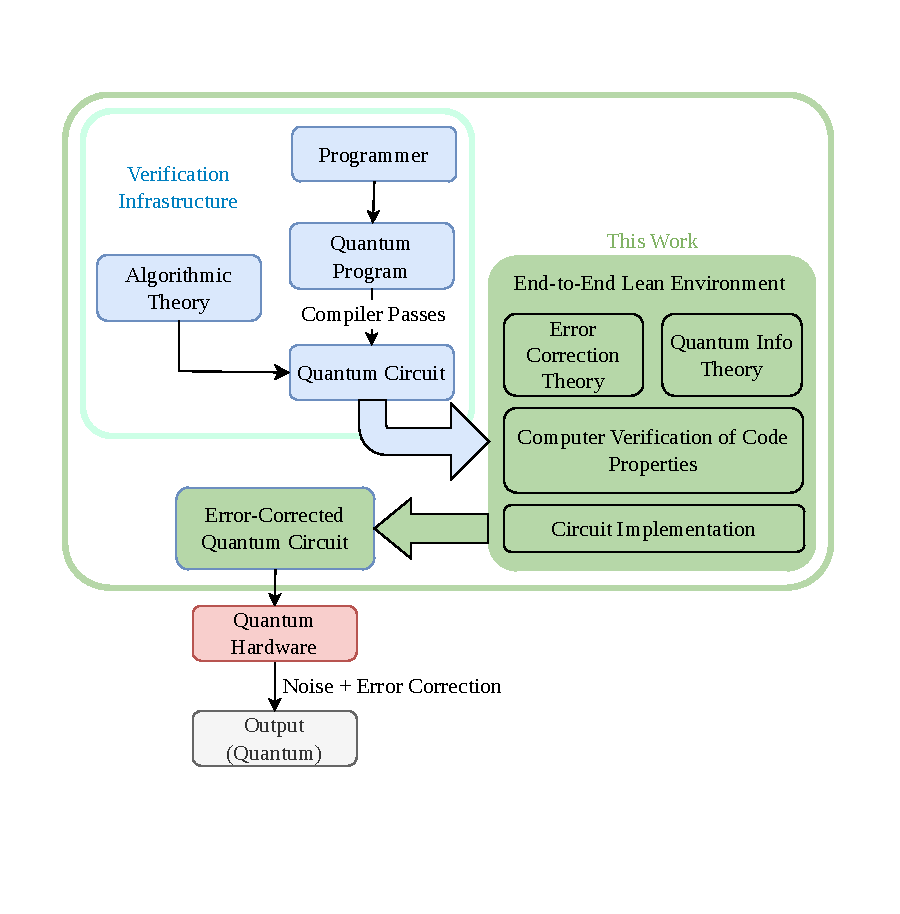
\includegraphics[width=0.9\linewidth]{Figures/qflow.drawio.pdf}
    \vspace{-2cm}
    \caption{Verification workflow for fault-tolerant quantum programs.
    \textsc{Lean-QEC} occupies the QEC layer of this pipeline.}
    \label{fig:qflow}
\end{figure}

\begin{table}[ht]
\small
\centering
\caption{Comparison of verification approaches for QEC
distance.}\label{tab:comparison}
\begin{tabular}{@{}lccc@{}}
\toprule
\textbf{Approach} & \textbf{Theory verified?} & \textbf{Scales to large codes?} & \textbf{End-to-end checked?} \\
\midrule
Hand-written ITP proofs         & Yes & No ($n > 20$ prohibitive) & Yes \\
Unverified symbolic computation & No  & Yes                       & No  \\
\textsc{Lean-QEC} (this work)   & Yes & Yes (${\sim}2^{40}$ cases) & Yes \\
\bottomrule
\end{tabular}
\end{table}


The rest of the paper develops \textsc{Lean-QEC} in the order a quantum
researcher would encounter the abstractions: \Cref{sec:fv} introduces just
enough Lean to follow the formalization; \Cref{sec:QECBackground} builds the QEC
stack with explicit attention to the type-theoretic gaps that arise when
formalizing standard quantum-information arguments; \Cref{sec:smt} presents the
SAT-assisted distance pipeline; \Cref{sec:casestudies} reports the case studies;
and \Cref{sec:Conclusion and Discussion} discusses related work and limitations.


%----------------------------------------------------------------------
\section{Background}\label{sec:setting}
%----------------------------------------------------------------------
\label{sec:fv}

% Lean~4~\cite{demoura2021} is an interactive theorem prover and programming
% language built on a theory known as the Calculus of Inductive Constructions.
% Essentially, this allows it to represent mathematical structures and arguments
% in type theory (as opposed to the standard Set Theory) and verify the
% correctness of statements. Once Lean has verified that a statement is correct,
% to be fully confident in its output you must only believe two things:
%
% \begin{enumerate}[leftmargin=1.5em]
%     \item That the formal statement in Lean is equivalent to the informal
% counterpart
%     \item That Lean's small, independently verified proof kernel is correct.
% \end{enumerate}
% Thus, verifying mathematical statements in Lean gives you significantly more
% confidence in the truth of the statement. So long as the statements match,
% there is no need for a human to check the arguments used to prove the
% statements.
%
% One of the main reasons for using Lean is its robust and wide-ranging Mathlib
% library, which provides nearly 2 million lines of code across many branches of
% mathematics. Mathlib is able to define an increasing amount of research
% mathematics, and underpins all major Lean formalization projects like the
% Prime Number Theorem \cite{Kontorovich_Prime_Number_Theorem_2024} and Fermat's
% Last Theorem projects \cite{FLT_Lean}. For our project, Mathlib provides a
% number of indispensable algebraic objects that support the theory of Quantum
% Error Collection, and any large Lean project must plan to have some of its
% work eventually adopted into Mathlib for use by others.
%
% To provide an intuition on interactive theorem proving, we will sketch one of
% our lemmas and provide a side-by-side comparison with the Lean formalization.
% In general, Lean formalizations follow the same structure as pen-and-paper
% arguments, except all minor details must be fleshed out.
% For example, while formalizing code distances,
% since we cannot take a minimum over the empty set,
% we must explicitly handle an edge case for when there are no undetectable
% Pauli errors.
% (That is, when the only valid codeword is $0^n$.)
% Concretely, we define the \emph{distance} of a quantum error correcting code
% as follows.
%

This section gives some background Lean and formal verification for
\Cref{sec:QECBackground,sec:smt}. We assume familiarity with quantum error
correction and standard linear algebra.
For more details please refer to \cite{avigad2020mathematics}.

\paragraph{Lean 4 and Mathlib.} Lean~4~\cite{demoura2021} is an interactive
theorem prover (ITP) and a dependently typed functional programming language
whose underlying logic is the Calculus of Inductive Constructions. Statements
and proofs are both first-class objects: a proof of a proposition $P$ is a value
whose type is $P$. Once Lean has accepted a proof, the only assumptions a reader
needs to discharge are (i)~that the Lean statement faithfully captures the
intended informal claim and (ii)~that Lean's small, independently audited kernel
is correct.

The standard library \emph{Mathlib}~\cite{mathlib2020} now contains close to two
million lines of formalized mathematics and underpins large efforts such as the
Prime Number Theorem~\cite{Kontorovich_Prime_Number_Theorem_2024} and Fermat's
Last Theorem~\cite{FLT_Lean} projects. We rely on Mathlib for matrices,
finite-dimensional vector spaces, group theory, unitary groups, and the
Kronecker product; conversely, our development is designed to be portable back
into Mathlib as quantum-information content matures there.

\paragraph{Formalizing Math with an ITP.} A Lean proof is a sequence of \emph{tactics} that incrementally transforms the goal, and any informal pen-and-paper argument can be translated by spelling out the steps the human reader would otherwise fill in. The friction sits in those omitted steps: edge cases that the prose dismisses with ``clearly,'' implicit coercions between mathematically equivalent representations, and definitions whose set-theoretic phrasing is awkward in type theory.

\begin{mybox}{\textbf{Example: Proving Distance in Lean}}

For a concrete Lean example we revisit a definitional edge case that arises in our own
development. The distance of a quantum error-correcting code is the minimum
Pauli weight of an undetectable error, but a minimum over the empty set is
undefined; we must pick a convention for codes whose only valid codeword is
$0^n$. We follow the standard ``$n+1$'' convention, which makes the distance
well-defined while reserving the literal value $n+1$ as a sentinel for the
trivial case.

\textbf{Definition:} Given an error-correcting code $\mathsf{C}$, let $S\subseteq \mathbb{P}_n$
    be the set of undetectable Pauli errors.
    We then define the distance by
    \begin{equation}
        d = \begin{cases}
            \min_{P\in S}(\mathsf{weight}(P)) & \textnormal{if } S\ne\emptyset \\
            n+1 & \textnormal{if } S = \emptyset
        \end{cases}
    \end{equation}


The sentinel value makes the following sanity check immediate, but only
\emph{after} the case split is made explicit.

\textbf{Lemma:} If the distance $d$ of a code over $n$ qubits satisfies $d \leq n$, then its
    set $S$ of undetectable errors is nonempty.
\begin{proof}
    Suppose $S = \emptyset$ for contradiction. By the definition of code distance, we
    have $d = n+1$, contradicting $d \leq n$.
\end{proof}

A corresponding Lean proof mirroring step-by-step the above informal argument would be written as:

\begin{lstlisting}
lemma BinSympMatrix.undetectable_set_nonempty {k n : ℕ}
    (B : BinSympMatrix k n) (hk : 0 < k)
    (h_dist : B.distance hk ≤ n) :
  B.undetectable_set.Nonempty := by
  by_contra h_empty
  rw [Finset.not_nonempty_iff_eq_empty] at h_empty
  unfold BinSympMatrix.distance at h_dist
  rw [h_empty] at h_dist
  simp at h_dist
\end{lstlisting}    

This proof may be read as follows: \lstinline{by_contra} introduces the
contradiction hypothesis; \lstinline{Finset.not_nonempty_iff_eq_empty} converts
``non-emptiness'' into a Finset-level equation that Mathlib has lemmas about;
\lstinline{unfold} and \lstinline{rw} apply the definition and the empty-set
hypothesis; \lstinline{simp} discharges the residual arithmetic against $d \le
n$. The mechanical overhead, which involves naming the empty-set lemma and finding the right lemmas to rewrite with, is representative of what formalizing a pen-and-paper QEC
argument feels like in practice. 


\end{mybox}


%
% Lean proofs are composed of a series of "tactics", which perform mathematical
% proof techniques like deductive logic identities, syntactic rewriting, and
% more complex simplification procedures. The theorem is stated as:
%
% \begin{lstlisting}
%     theorem dual_dual_eq {C : CodeSpace n} : (C.dualCode).dualCode = C
% \end{lstlisting}
%
% As an Interactive Theorem Prover, Lean provides a ``context window`` the
% displays the user's slate of current hypotheses, and the ``goal'' they are
% trying to prove in the proof environment. For this theorem, it looks like:
%
% \begin{lstlisting}
% n : ℕ
% C : CodeSpace n
% ⊢ C.dualCode.dualCode = C
% \end{lstlisting}
%
% We plan to prove it by way of the Mathlib lemma
% \lstinline{Submodule.eq_of_le_of_finrank_eq}, which has statement:
%
% \begin{lstlisting}
% Submodule.eq_of_le_of_finrank_eq.{u, v} {K : Type u} {V : Type v}
%   [DivisionRing K] [AddCommGroup V] [Module K V]
%   {S₁ S₂ : Submodule K V} [FiniteDimensional K ↥S₂] (hle : S₁ ≤ S₂)
%   (hd : Module.finrank K ↥S₁ = Module.finrank K ↥S₂) :
%   S₁ = S₂
% \end{lstlisting}
%
% This may be read as follows: beginning with \lstinline|{K : Type u}| are the
% arguments for the lemma, which requires types \lstinline{K} and \lstinline{U}
% with \lstinline{K} being a Division Ring, and \lstinline{V} being a
% commutative module over $K$. With types specified, submodules \lstinline{S₁, % S₂} are then
% defined, and \lstinline{S₂} is required to be finite dimensional.
% The two main hypotheses are that \lstinline{S₁} is a submodule of
% \lstinline{S₂}, and that \lstinline{S₁} and \lstinline{S₂} have equal rank.
% After the colon is the ``type'' of the lemma, or the proposition it
% ``produces'' a proof object for (by the Curry-Howard isomorphism, Lean proofs
% are functions in a functional programming language).
% \Ethan{I feel like either the reader already knows Curry-Howard or they don't.
% In the latter case, we have no chance of successfully conveying the idea.}
% Note that the lemma arguments are variously provided in square brackets, curly
% braces, and parentheses. The parentheses-closed arguments are explicitly
% provided to the function, while the remainder of the arguments are
% automatically synthesized.
%
% Running the following tactics:
%
% \begin{lstlisting}
% symm
% apply Submodule.eq_of_le_of_finrank_eq
% \end{lstlisting}
%
% First reverses the order of the equality in the goal, then ``applies'' the
% lemma, synthesizing its arguments with the goal and seeking explicit
% instantiations of the goal's arguments. The context window then looks like:
%
% \begin{lstlisting}
% 2 goals
% case hle
% n : ℕ
% C : CodeSpace n
% ⊢ C ≤ C.dualCode.dualCode
% case hd
% n : ℕ
% C : CodeSpace n
% ⊢ Module.finrank (ZMod 2) ↥C = Module.finrank (ZMod 2) ↥C.dualCode.dualCode
% \end{lstlisting}
%
% To dispatch the first goal, we need to prove that \lstinline{S ≤ % S.dualCode.dualCode}.
% \Ethan{I feel anything beyond this is too much.
% We should probably refer to some standard course/textbook instead.
% We aren't here to teach the readers how interactive theorem provers work.}
% An earlier definition specifies the dual as the orthogonal submodule with
% respect to the dot product, so we apply another Mathlib lemma about submodules
% defined as:
%
% \begin{lstlisting}
% Submodule.le_orthogonalBilin_orthogonalBilin.{u_1, u_2, u_5, u_6} {R : Type
% u_1} {R₁ : Type u_2} {M : Type u_5}
%   {M₁ : Type u_6} [CommRing R] [CommRing R₁] [AddCommGroup M₁] [Module R₁ M₁]
% [AddCommGroup M] [Module R M]
%   {I₁ I₂ : R₁ →+* R} {B : M₁ →ₛₗ[I₁] M₁ →ₛₗ[I₂] M} {N : Submodule R₁ M₁} (b :
% B.IsRefl) :
%   N ≤ (N.orthogonalBilin B).orthogonalBilin B
% \end{lstlisting}
%
% The other goal about equal rank is proved using an earlier lemma defining the
% rank of the dual code, \lstinline{dual_finrank_eq}.
%
% \begin{lstlisting}
% lemma dual_finrank_eq {C : CodeSpace n} : Module.finrank (ZMod 2) C.dualCode =
% n - (Module.finrank (ZMod 2) C)
% \end{lstlisting}
%
% Rewriting this twice, the goal is now:
%
% \begin{lstlisting}
% ⊢ Module.finrank (ZMod 2) ↥C = n - (n - Module.finrank (ZMod 2) ↥C)
% \end{lstlisting}
%
% Which is proven by simplification tactics after asserting that \lstinline{C}
% has rank at most $n$, as the subtraction is occurring over the natural numbers
% and would be false otherwise.
%
%

%This example demonstrates Lean's expressive power as well as the benefits
%gained from working with Mathlib.

%\subsection{Satisfiability Modulo Theories}

%\emph{Satisfiability modulo theories} (``SMT'') is a natural generalization of
%the Boolean satisfiability (``SAT'') problem.
%Instead of working with only Boolean variables, SMT allows formulas to include
%various data types and structures.
%Similar to SAT, SMT is NP-hard in general,
%thus SMT instances are usually treated using specialized solvers such as cvc5
%\cite{barbosa2022}, alt-ergo \cite{conchon2018alt}, and Z3 \cite{de2008z3}.
%The comparisons and inner workings of these solvers are out of the scope of our
%discussions.
%For the purpose of our project,
%we will treat solvers as black-boxes that run in (at worst) asymptotically
%exponential time.

%Most popular proof assistant software include various levels of solver support.
%In Lean, we use CaDiCaL \cite{biere2024cadical} for SAT instances, and Lean-SMT
%(based on cvc5) \cite{mohamed2025lean} for SMT instances.
%In these integrations,
%the solver should ideally not be included within the trusted computing base
%(TCB).
%Instead, the solver could return proofs of (un)satisfiability, which are then
%translated and verified using standard techniques such as Curry-Howard
%isomorphism. For cvc5, the standard solver contains a flag which causes it to
%return a "proof" of its reasoning in the Cooperating Proof Calculus (CPC),
%which may be verified by its checker Ethos and is compatible with the Eunoia
%framework. Unfortunately, this translation step from proof calculi to Lean, due
%to the overhead of being performed within Lean, becomes computationally
%prohibitive for larger and more complex SMT instances.
%As a result, frameworks such as EasyCrypt have chosen to absorb their solvers
%into their TCB, and to accept their external solvers' outputs without
%verification.

%On the proof engineering side, SMT solvers are often treated similarly to
%\emph{hammer} tactics.
%In other words, they are designed for goals that seem more tedious than
%complex.
%As a result, it is conventional to set a timeout of well under one minute per
%SMT invocation.
%As we discuss in \Cref{sec:smt} however,
%some of our project's goals require hours-long SMT runs.


%----------------------------------------------------------------------
\section{Formalization of Quantum Error Correction}\label{sec:QECBackground}
%----------------------------------------------------------------------

\begin{figure}[!b]
    \centering
    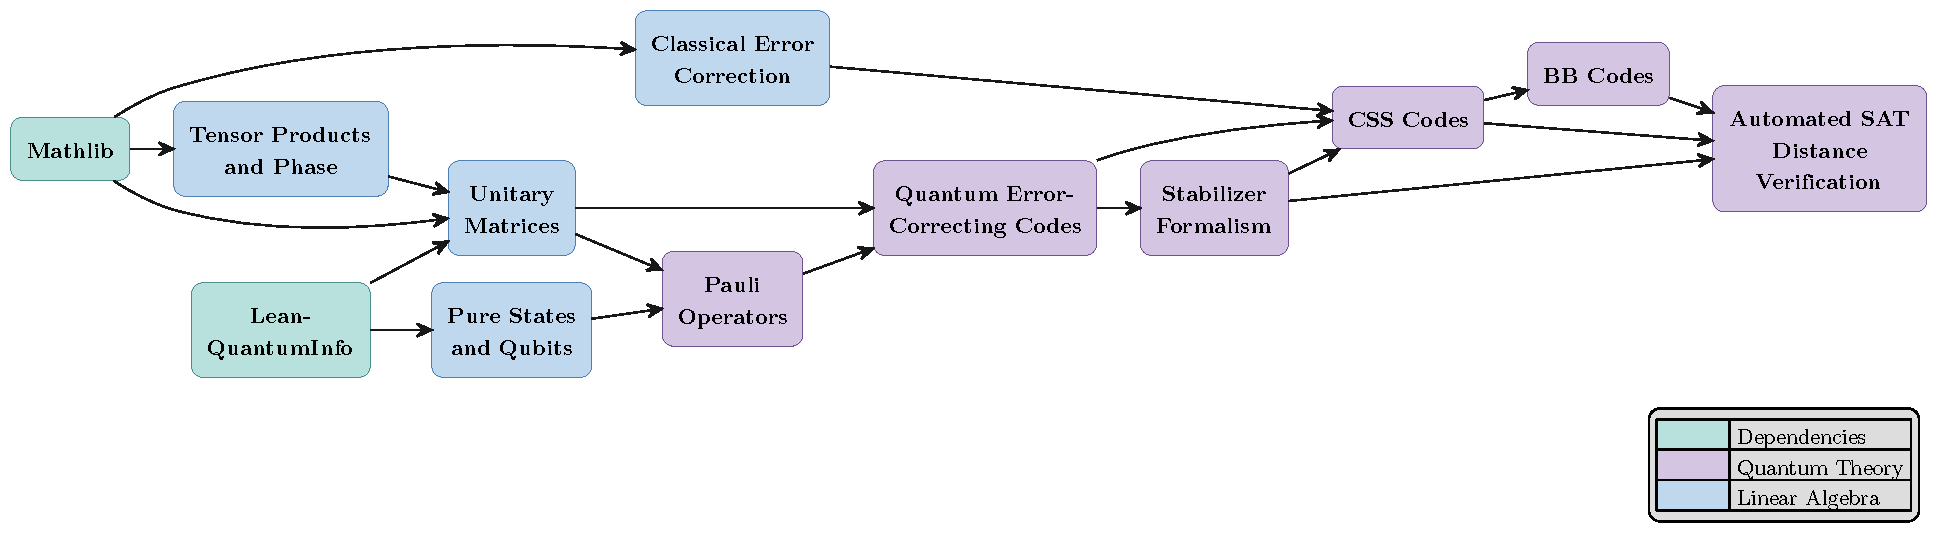
\includegraphics[width=\linewidth]{Figures/fig3_theory_map.pdf}
    \caption{Map of the formalized quantum-error-correction stack. Arrows are
    machine-checked correspondence theorems; the rightmost layer feeds into the
    SAT-based distance pipeline of \Cref{sec:smt}.}
    \label{fig:qmap}
\end{figure}

% To demonstrate the interesting challenges faced in formalizing Quantum Error
% Correction and compare writing in Lean to informal mathematical writing, we
% will present background and formalization simultaneously. In \ref{fig:qmap},
% we map the major accomplishments of the theory and how they relate to each
% other. The major accomplishments of the repository are the theorems proved
% relating the distance of Quantum Error-Correcting Codes to the linear
% algebraic and boolean versions of the statements, and most parts of the
% repository are leading towards those results.
%

This section builds the stack from \Cref{fig:qmap} bottom-up: qubit states,
$n$-qubit unitaries, the Pauli group with phases, the binary symplectic
representation, abstract QEC codes, stabilizer codes, and finally the CSS and
Bivariate Bicycle families. For each layer we describe the formalization choice,
the machine-checked correspondence to the layer below, and the type-theoretic
friction that distinguishes the Lean development from a pen-and-paper account.
The chain of correspondences ending at the binary symplectic matrix is what
makes the SAT-based distance pipeline of \Cref{sec:smt} end-to-end: a distance
bound discharged at the bottom transports, by a Lean theorem, to a bound on the
quantum code at the top.

\subsection{Qubit States}
\label{sec:qc}

% We begin with our formalization of quantum states.
% Formalization of quantum algorithms have been studied by the SQIR line of
% literature \cite{hietala2021} as well as CoqQ \cite{coqq}.
% Unfortunately, as they are formalized using a different proof assistant,
% we do not have an easy way to make use of them.
% On the other hand, the Lean-QuantumInfo \cite{leanquantuminfo} project does
% not specialize its quantum states to the qubit space, so this is where our
% formalization starts.
%
% When we are asked to define a $n$-qubit state, the first answer is perhaps a
% $2^n$-dimensional vector over $\bbC$.
% On the other hand, when we are asked to write down the general form of a
% quantum state $\ket{\psi}$, we often write the expression
% $$\ket{\psi}=\sum_{x\in\set{0, 1}^n}\alpha_x\ket{x}.$$
% Now, the $n$-qubit standard basis, indexed using $n$-bit binary strings, is
% certainly isomorphic to the space $\bbC^{2^n}$, simply by collecting all the
% amplitudes $\alpha_x$.
% This syntactic mismatch, and equivalence up to isomorphism, however, represent
% a design decision that we must make through our proof engineering.
%
% In Lean, vectors of the form $\mathbb{F}^n$ are conventionally formalized
% using the property
% \begin{equation}
%     \label{eq:vec-equiv-fn}
%     \mathbb{F}^n\cong \Fun(\bbN_n, \mathbb{F})
% \end{equation}
% where $\bbN_n=\set{0, 1, \ldots, n-1}$ denotes the set of natural numbers up
% to $n$.
% Perhaps this is unsurprising, since $Y^X$ is the standard notation for the set
% of functions $\Fun(X, Y)$ in many mathematics communities.
% We follow the same conventions and formalize our quantum state by
% $\Fun(\set{0, 1}^n, \bbC)$
% up to the usual amplitude normalization constraints;
% that is, we would write $\mathbb{C}^{\set{0, 1}^n}$, instead of
% $\mathbb{C}^{2^n}$ like in other verified frameworks such as SQIR.
% One benefit of our formalism is that it allows us to treat tensor products
% more naturally.
% For example, suppose we have two standard basis states, $\ket{101}$ and
% $\ket{001}$.
% To combine them then, we would write
% $$\ket{101}\otimes\ket{001}=\ket{101001},$$
% simply concatenating the two strings together.
% On the other hand, in formalizations using $2^n$-dimensional vectors instead,
% taking the product between qubit states would involve bit-shifting the
% operands, which may be more tedious to analyze.
%

The SQIR development~\cite{hietala2021} and CoqQ~\cite{coqq} formalize quantum
states in Rocq Prover, and the Lean-QuantumInfo project~\cite{leanquantuminfo}
formalizes general finite-dimensional quantum states in Lean. None of these
specialize the state space to qubits in the way we need, so we start the stack
ourselves.

\paragraph{Choice of index set.} A textbook quantum researcher writes a pure
state as
$\ket{\psi} = \sum_{x \in \{0,1\}^n} \alpha_x \ket{x}$,
i.e.\ as an assignment of amplitudes to bit strings. A textbook formalizer
writes it as an element of $\mathbb{C}^{2^n}$. The two views are isomorphic, but
Lean represents a finite-dimensional vector by its function form
\begin{equation}
    \label{eq:vec-equiv-fn}
    \mathbb{F}^n \cong \Fun(\bbN_n, \mathbb{F}), \qquad \bbN_n = \{0, 1, \ldots, n-1\},
\end{equation}
and the choice of index set is a load-bearing design decision: every later
definition is parametrized by it. We diverge from SQIR's $\mathbb{C}^{2^n}$
convention and adopt $\Fun(\{0,1\}^n, \mathbb{C})$, written
$\mathbb{C}^{\{0,1\}^n}$ with the usual normalization. The payoff is that
tensor products on basis states become string concatenation, $\ket{101} \otimes
\ket{001} = \ket{101001}$, instead of an arithmetic identity on bit-shifts; this
matters because Pauli operators are most naturally indexed by which qubit they
act on, not by a position in a flattened $2^n$-array.

\subsection{Quantum Operators}

% There are many sophisticate and powerful formalizations of quantum operations.
% These existing frameworks have had to face many challenges, type-theoretic and
% otherwise, in order to describe circuit-like constructions:
% for example, to add a two-qubit gate on the $i$-th and $j$-th qubits in an
% $n$-qubit system.
% For our purpose of studying quantum error correction,
% we will avoid re-inventing those wheels, and leave fleshing out such a
% framework in Lean for future work.
% For quantum error corrections, it would suffice if we can ``glue'' states and
% operators together consistently.
% In particular, we have to verify that for all states $\ket{\phi_1}$ and
% $\ket{\phi_2}$, and all operators $U_1$ and $U_2$,
% we have
% \begin{equation}
% \label{eq:kron-ustate}
% (U_1\otimes U_2)(\ket{\phi_1}\otimes\ket{\phi_2})=U_1\ket{\phi_1}\otimes
% U_2\ket{\phi_2}.
% \end{equation}
%
% As simple as \Cref{eq:kron-ustate} may seem,
% there is already a gap that we must address carefully.
% Colloquially, we often use the term \emph{tensor product} for both products
% between quantum states and between operators.
% (In fact, we used the same symbol for them in \Cref{eq:kron-ustate}.)
% Technically speaking, however, we should use the term \emph{tensor product}
% for the product between vectors, and the more general \emph{Kronecker product}
% for matrices.
% These two notions indeed correspond to two different functions in Mathlib.
% In order to avoid the deep Mathlib abstractions involving connections between
% tensor and Kronecker products,
% we will simply formalize all the ``tensor'' products as Kronecker products,
% in such a way that \Cref{eq:kron-ustate} matches one of the Mathlib lemmas.
%
% We begin with a sketch of Mathlib's formalization of matrices and Kronecker
% products.
% Similarly to how vectors are isomorphic to functions as given by
% \Cref{eq:vec-equiv-fn},
% we have a similar isomorphism for matrices for all natural numbers $m,
% n\in\bbN$:
% \begin{equation}
%     \label{eq:mat-eq-fn}
%     \mathbb{F}^{m\times n}\cong\Fun(\bbN_m\times\bbN_n, \mathbb{F})
% \end{equation}
% That is, roughly speaking, matrices are characterized by a collection of ring
% elements indexed by the Cartesian product between two sets.
% Now, Kroneckers products are then defined by Mathlib as follows.
% \begin{definition}[Kronecker product, Mathlib]
%   Let $I_1, I_2, J_1, J_2$ be arbitrary sets, and let $\mathbb{F}$ be a ring.
%   Let $M_1\in\mathbb{F}^{I_1\times J_1}$ and $M_2\in\mathbb{F}^{I_2\times
% J_2}$ be matrices.
%   The \emph{Kronecker product} of $M_1$ and $M_2$ is then identified by the
% function $M_1\otimes M_2:(I_1\times I_2)\times(J_1\times J_2)\rightarrow
% \mathbb{F}$ where
%   \begin{equation}
%       (M_1\otimes M_2)((i_1, i_2), (j_1, j_2)) = M_1(i_1, j_1)\cdot M_2(i_2,
% j_2).
%   \end{equation}
% \end{definition}
%
% Now, this definition immediately introduces some interface mismatches for the
% purpose of operations over qubits.
% For instance, suppose $U_1$ is an $n_1$-qubit operator, and $U_2$ is an
% $n_2$-qubit operator.
% Conceptually then, their product $U_1\otimes U_2$ should act on $n_1+n_2$
% qubits.
% Stepping through the definitions so far, however, $U_1$ would be of the type
% $U_1\in\bbC^{\set{0, 1}^{n_1}\times\set{0, 1}^{n_1}}$, and similary for $U_2$.
% Their tensor product then yields the type
% \begin{align}
% U_1\otimes U_2&\in
% \bbC^{(\set{0, 1}^{n_1}\times\set{0, 1}^{n_2})\times(\set{0,
% 1}^{n_1}\times\set{0, 1}^{n_2})})\\
% &\cong\Fun((\set{0, 1}^{n_1}\times\set{0, 1}^{n_2})\times(\set{0,
% 1}^{n_1}\times\set{0, 1}^{n_2}), \bbC)
% \end{align}
% instead of the desired type
% $$\bbC^{\set{0, 1}^{n_1+n_2}\times\set{0, 1}^{n_1+n_2}})\cong
% \Fun((\set{0, 1}^{n_1+n_2}\times \set{0, 1}^{n_1+n_2}), \bbC).$$
% In other words, we are left with a gap in the shape of the isomorphism
% $$\set{0, 1}^{n_1}\times\set{0, 1}^{n_2}\cong\set{0, 1}^{n_1+n_2}.$$
% That is, the Cartesian product of two bit-strings is equivalent to their
% concatenation,
% which is a mismatch that we must fill in.
% Similarly, in order to specialize the Kronecker products and recover the
% tensor product between vectors, it remains to layer yet another isomorphism on
% top, allowing ourselves to explicitly convert between $n$-dimensional vectors
% and size $n\times 1$ matrices.
%
% It is worth noting that in our formalization so far, we have already faced
% some of the type-theoretic challenges as with the CoqQ project.
% In particular, consider the following lemma:
% \begin{lemma}
%     \label{lem:kron-assoc}
%     Let $U_1$ be an operator acting on $n_1$ qubits,
%     and similarly for $U_2$ with $n_2$ and $U_3$ with $n_3$.
%     We then have
%     \begin{equation}
%         (U_1\otimes U_2)\otimes U_3=U_1\otimes(U_2\otimes U_3)
%     \end{equation}
% \end{lemma}
%
% In the context of the dependent type systems of Lean (and of Rocq Prover),
% the lemma statement is in fact \emph{ill-typed}.
% That is because the left-hand side acts on $(n_1+n_2)+n_3$ qubits, and the
% right-hand side acts on $n_1+(n_2+n_3)$ qubits;
% the issue being that the equality $(n_1+n_2)+n_3=n_1+(n_2+n_3)$ is a
% \emph{semantic} property which the type checker cannot make direct use of.
% We stress that the difficulty is not in that we cannot \emph{prove}
% \Cref{lem:kron-assoc}, but that the Lean compiler does not even accept the
% lemma statement itself.
% Historically speaking, formalizations of quantum computations have taken
% different workarounds for this issue.
% Luckily, Lean's Mathlib allows the use of \emph{heterogenous equalities},
% which is perhaps the most elegant solution by far.
% In short, heterogenous equalities allow programmers to first assert and prove
% that the left-hand-side and right-hand-side of an equation are of equal type,
% and then the compiler accepts the proof script as well-typed.
%
% Finally, the astute reader may have noticed that we have discussed about
% matrices so far, but not much of unitary operators yet.
% Fortunately, unitary operators and their properties are already formalized in
% Lean's Mathlib, and are indeed used extensively by both the Lean-QuantunInfo
% project and ourselves.
% We remark that this does not introduce any additional conceptual challenges,
% but only more boilerplate code that we have also written.
%

For the purpose of QEC we do not need a full circuit DSL; we only need to
compose states and operators consistently. The single property we require is
\begin{equation}
\label{eq:kron-ustate}
(U_1 \otimes U_2)(\ket{\phi_1} \otimes \ket{\phi_2}) = (U_1 \ket{\phi_1}) \otimes (U_2 \ket{\phi_2}),
\end{equation}
together with associativity of $\otimes$ on operators. The Lean development for
a richer gate-level circuit calculus is left to future work.

\paragraph{Tensor vs.\ Kronecker.} \Cref{eq:kron-ustate} hides a vocabulary
issue. The product on states is a \emph{tensor product} of vectors; the product
on operators is a \emph{Kronecker product} of matrices. Mathlib distinguishes
them as two different functions, and the abstract isomorphism connecting the two
passes through tensor-algebra machinery we would otherwise have to drag through
every proof. We sidestep this by formalizing every ``$\otimes$'' in our
development as a Kronecker product, with vectors viewed as $n \times 1$ matrices
when needed. This makes \Cref{eq:kron-ustate} a direct corollary of a Mathlib
lemma rather than a tour through Mathlib's tensor-algebra hierarchy.

\paragraph{Index alignment.} Matrices in Mathlib are functions on index pairs,
\begin{equation}
    \label{eq:mat-eq-fn}
    \mathbb{F}^{m \times n} \cong \Fun(\bbN_m \times \bbN_n, \mathbb{F}),
\end{equation}
and Mathlib's Kronecker product is defined accordingly: for $M_1 \in
\mathbb{F}^{I_1 \times J_1}$ and $M_2 \in \mathbb{F}^{I_2 \times J_2}$,
\begin{equation}
    (M_1 \otimes M_2)((i_1, i_2), (j_1, j_2)) = M_1(i_1, j_1) \cdot M_2(i_2, j_2).
\end{equation}
For an $n_1$-qubit operator $U_1$ and an $n_2$-qubit operator $U_2$, the index
type produced by this definition is $\{0,1\}^{n_1} \times \{0,1\}^{n_2}$,
whereas the index type of an $(n_1+n_2)$-qubit operator is $\{0,1\}^{n_1+n_2}$.
The two are equal up to the isomorphism $\{0,1\}^{n_1} \times \{0,1\}^{n_2}
\cong \{0,1\}^{n_1+n_2}$ that concatenates bit strings, but Lean's dependent
type system does not coerce them implicitly. We discharge this gap by a one-time
concatenation/splitting bijection; every later lemma uses operators indexed by
$\{0,1\}^{n}$ uniformly.

\paragraph{Heterogeneous equality.} Associativity of $\otimes$ on operators, $(U_1 \otimes U_2) \otimes U_3 = U_1
    \otimes (U_2 \otimes U_3)$,
is well-formed on paper but not in Lean: the LHS has type indexed by
$(n_1+n_2)+n_3$ qubits and the RHS by $n_1+(n_2+n_3)$, and $\mathbb{N}$'s
addition is not associative \emph{definitionally}. Other formalizations work
around this with explicit cast functions sprinkled through every proof. Lean's
Mathlib provides a cleaner option, \emph{heterogeneous equality}: the equation
is stated between values of provably-equal types, and the type checker accepts
it once the type-level equality has been discharged. We use this idiom
throughout the development.

\paragraph{Unitarity.} Mathlib already supplies the unitary-group structure on
square matrices, and Lean-QuantumInfo uses it as well; we inherit it directly.
Wrapping our Kronecker-based operators in Mathlib's unitary group introduces no
additional conceptual challenges, only boilerplate that we have written once.

% We are mostly concerned with accumulation of errors on Pure States here.
% Informally, a pure state written $\ket{\psi}$ is defined as a vector in
% $\mathbb{C}^{2^n}$ with $\ell_2$-norm of $1$, meaning that:
% \begin{equation}
%     \sum_{x \in \{0, 1\}^n} |\ket{\psi}_x|^2 = 1
% \end{equation}
%
%
% \Ethan{I wonder if it's worth presenting everything we have in terms of pure
% states first, before talking about unitaries operators in general.
% For example, we can say we're using $$\mathbb{C}^{\set{0,
% 1}^n}\cong\Fun(\set{0, 1}^n, \mathbb{C})$$instead of $\mathbb{C}^{2^n}$.}
%
% A Quantum State evolves from $\ket{\psi} \mapsto \ket{\psi'}$ according to
% some \textbf{Unitary Matrix}, which on $n$ qubits is $U \in
% M_{2^n*2^n}(\mathbb{C})$ such that $U^*=U^{-1}$, where $U^*$ is the conjugate
% transpose.
%
% Formaly, we begin with a general pure state definition, defining the vector as
% indexed over some finite type \lstinline{d}, as opposed to fixed qubit sizes.
% Due to building off Lean's \textit{Mathlib} library, we are able to use a
% prepackaged definition of unitary matrices.
%
% \begin{lstlisting}
% variable (d : Type*) [Fintype d]
% structure Ket where
%   vec : d → ℂ
%   normalized' : ∑ x, ‖vec x‖ ^ 2 = 1
%
% notation "U[" n "]" => Matrix.unitaryGroup n ℂ
% \end{lstlisting}
%
% However, our focus on qubits means we are best served specializing our
% definitions like so:
%
% \begin{lstlisting}
% abbrev PState (n : ℕ) := Ket (BitVec n)
%
% notation "Uₙ[" n "]" => Matrix.unitaryGroup (BitVec n) ℂ
%
% \end{lstlisting}
%
% It is important to note that a Matrix, according to Mathlib, is a function
% with type signature \lstinline{l → m → α}. This is interpreted as a function
% taking inputs of type \lstinline{l} and \lstinline{m}, outputting a value of
% type \lstinline{α}. The value of type \lstinline{l} represents the index of
% the row of the matrix, while \lstinline{m} represents the column index and
% \lstinline{α} the element type.
%
% Quantum computing natively uses the tensor product, which is informally
% defined on vectors and matrices as allowing "multiple indexing". The tensor
% product $A \otimes B$, where $A$ is indexed by $r_1, c_1$ and $B$ is indexed
% by $r_2, c_2$, then $(A \otimes B)$ will be indexed by $r_1 \times r_2, c_1
% \times c_2$, with $(A \otimes B)_{a_1a_2, b_1b_2} = A_{a_1, b_1} * B_{a_2,
% b_2}$. Mathlib defines the kronecker product of matrices through
% \lstinline{kroneckerMap}, defined:
%
% \begin{lstlisting}
% def kroneckerMap (f : α → β → γ) (A : Matrix l m α) (B : Matrix n p β) :
% Matrix (l × n) (m × p) γ :=
%   of fun (i : l × n) (j : m × p) => f (A i.1 j.1) (B i.2 j.2)
% \end{lstlisting}
%
% Essentially, it takes matrices with rows indexed by type \lstinline{l} and
% \lstinline{n}, columns indexed by type \lstinline{m} and \lstinline{p}, and
% outputs a matrix with rows indexed by \lstinline{(l × n)} and columns by
% \lstinline{(m × p)}. If we then take the tensor product of two objects of type
% \lstinline{Uₙ[n]}, the output type of \lstinline{Matrix.kronecker} will be
% \lstinline{Matrix (Bitvec n × BitVec n) (Bitvec n × BitVec n) ℂ}. However, we
% want its type to be \lstinline{Matrix (BitVec (2*n)) (BitVec 2*n)}. Of course,
% these two types are roughly equivalent, as a \lstinline{BitVec 2*n} can be
% seen as containing two \lstinline{BitVec n} values. Thus, they are isomorphic,
% with a bijection acting as concatenation and splitting. Faced with explicitly
% applying this mapping every time, we instead choose to specialize our tensor
% product by composing it with this bijection, with type signature:
%
% \begin{lstlisting}
% def unitary_nkron {n₁ n₂ : ℕ} (a : Uₙ[n₁]) (b : Uₙ[n₂]) : Uₙ[n₁ + n₂]
% \end{lstlisting}
%
% We specialize similarly out tensor product for \lstinline{PState n}. 
%
% \begin{lstlisting}
% def PState.kron {n₁ n₂ : ℕ} (ψ₁ : PState n₁) (ψ₂ : PState n₂) : PState (n₁ +
% n₂)
% \end{lstlisting}
%
%

\subsection{Pauli Group}

% In many standard analyses, quantum errors are first decomposed into
% \emph{Pauli} operators.
% We formalize the structures and properties of the Pauli group accordingly.
% Pauli operators are often\footnote{e.g. Pauli one-time pad in quantum
% cryptography} characterized by expressions of the form $X^xZ^z$, where $x,
% z\in\set{0, 1}^n$ are classical strings of the same length as the number of
% qubits $n$.
% Operationally speaking, this corresponds to applying the single-qubit $X$-gate
% (resp. $Z$-gate) on each of the $i$-th qubits where $x_i=1$ (resp. $z_i=1$).
% This description of Pauli group is convenient for many pen-and-paper
% arguments.
% For example, the tensor product of two Pauli operators corresponds to string
% concatenation $X^{x_1}Z^{z_1}\otimes X^{x_2}Z^{z_2}=X^{x_1||x_2}Z^{z_1||z_2}$,
% and the ordinary matrix product becomes qubit-wise.
% As we will see in \Cref{sec:binsymp}, this characterization is also closely
% related to the \emph{binary symplectic representation} of Pauli operators.
%
% Unfortunately however, this $X^xZ^z$ characterization is both under-specified
% and inaccurate for the purpose of formal verification:
% \begin{itemize}
%     \item The Pauli operators are matrices that form a subset of
% $\mathbb{U}_{\set{0, 1}^n}$.
%     Currently, our informal description is described as a sequence of
% single-qubit operations, instead of a single matrix acting globally on the
% $n$-qubit space.
%     \item The informal description does not treat \emph{global phase} at all.
%     For example, we have the anti-commutation property $ZX=-XZ$, but the minus
% sign cannot be described by this $X^xZ^z$ formalism.
%     Moreover, the standard Pauli group should contain matrices such as
% $Y=-iXZ$, so even taking the multiplicative subgroup generated by $\langle X,
% Z\rangle$ does not suffice.
% \end{itemize}
% For the purpose of verification, we fill in these gaps in order to formalize
% the $X^xZ^z$-style argument rigorously.
% We begin by defining the single-qubit Pauli gates.
%

Quantum errors in our setting are decomposed into Pauli operators, so the Pauli
group is the first non-trivial structure in the QEC stack. The standard $X^x
Z^z$ shorthand --- ``apply $X$ to qubits with $x_i = 1$ and $Z$ to qubits with
$z_i = 1$'' --- is convenient for pen-and-paper arguments: the tensor product
becomes string concatenation, $X^{x_1}Z^{z_1} \otimes X^{x_2}Z^{z_2} = X^{x_1 \|
x_2}Z^{z_1 \| z_2}$, and the matrix product becomes qubit-wise. The same
shorthand also underlies the binary symplectic representation of
\Cref{sec:binsymp}.

\paragraph{What the shorthand omits.} Two gaps prevent us from using the $X^x
Z^z$ form directly as a Lean definition.
\begin{itemize}
    \item It describes a \emph{recipe} for building a unitary one qubit at a
    time, not a single matrix in $\mathbb{U}_{\{0,1\}^n}$. The Lean development
    needs the global matrix to state and prove e.g.\ commutation lemmas.
    \item It ignores global phase. The standard Pauli group contains $Y = -iXZ$
    and the anticommutation identity $ZX = -XZ$ depends on the sign; neither is
    expressible without phases. Restricting to the multiplicative subgroup
    $\langle X, Z\rangle$ does not recover $Y$.
\end{itemize}
We close both gaps explicitly. We start from the single-qubit Pauli matrices and
define a \emph{folding} function that turns a phase factor and an $n$-tuple of
single-qubit Paulis into a single $n$-qubit unitary. The Pauli group is then the
image of this function.
\begin{definition}[Single-qubit Pauli gates]
    \label{def:pauli-1}
    We define the following four unitary matrices (acting on the basis
    $\set{\ket{0}, \ket{1}}$) as the single-qubit Pauli gates.
    $$I = \begin{pmatrix}
    1 & 0 \\ 0 & 1
 \end{pmatrix}\quad X = \begin{pmatrix}
    0 & 1 \\ 1 & 0
\end{pmatrix}\quad Y = \begin{pmatrix}
    0 & -i \\ i & 0
\end{pmatrix} \quad Z = \begin{pmatrix}
    1 & 0 \\ 0 & -1
\end{pmatrix}$$
\end{definition}
% We next formalize ``folding'' these single-qubit Paulis into $n$-qubit
% operators.
% At the same time, here we allow adding a global phase of the form $i^a$ where
% $0\leq a\leq 3$.
%

The folding step assembles an $n$-tuple of single-qubit Paulis together with one
of the four phase factors $\{1, i, -1, -i\}$ into a single $n$-qubit unitary.
\begin{definition}[Pauli folding]
    \label{def:pauli-folding}
    For each $n \in \bbN$, define
    $$\PauliFold_n : \{1, i, -1, -i\} \times \{I, X, Y, Z\}^n \rightarrow
    \bbU_{\{0,1\}^n}$$
    by
    \begin{equation}
        \label{eq:def-pauli-fold}
        \PauliFold_n(\gamma, \vec{P}) = \gamma \cdot \bigotimes_i P_i.
    \end{equation}
\end{definition}
\begin{definition}
    \label{def:pauli-group}
    The $n$-qubit \emph{Pauli group} is the image of $\PauliFold_n$:
    \begin{equation}
        \label{eq:def-pauli-group}
        \bbP_n = \Image(\PauliFold_n).
    \end{equation}
\end{definition}
This is equivalent to the textbook definition. A common alternative is to
quotient by global phase and work with equivalence classes; we prefer the
image-of-fold form because it lets us write down a single matrix rather than a
coset representative, which keeps later proofs computable.

\begin{figure}
    \centering
    \begin{tikzcd}[column sep=large, row sep=large]
    P,\, P' \arrow{r} \arrow{d}{\mathsf{unfold}} &
    P \otimes P' \arrow{d}{\mathsf{unfold}} \\
    (\gamma, \{P_i\}_i),\, (\gamma', \{P_i'\}_i) \arrow[r] &
    (\gamma\gamma', \{P_i\}_i \doubleplus \{P_i'\}_i)
    \end{tikzcd}
    \caption{Tensor product of unfolded Pauli operators}
    \label{fig:pauli-commute}
\end{figure}

% With the Pauli group defined, next we formally verify the following (hopefully
% familiar) properties of Pauli groups.
% First, the mapping $\PauliFold$ defined by \Cref{eq:def-pauli-fold} is
% bijective.
% This in turn implies that each Pauli operator has a unique unfolded
% $\gamma\cdot X^xZ^z$ form.
% As we will see in \Cref{sec:distproblem}, this is crucial because the
% \emph{distance} of a quantum error correcting code depends on the \emph{Pauli
% weight} of the error considered.
% In other words, without unique unfolding, it is unclear whether the distance
% of a quantum error correcting code would be well-defined.
%
% Next, using the previous unique unfolding property, we verify that our
% $\PauliFold$ map respects tensor products and ordinary matrix products in the
% expected ways.
% In particular, the diagram given by \Cref{fig:pauli-commute} commutes for
% tensor product, and similarly for matrix product after collecting additional
% phase factors.
% This allows us to reason about Paulis using the $\gamma\cdot X^xZ^z$
% representation.
% (Along the way, we also verified several other low-level properties, such as
% that the Pauli group is closed under products.)
%
% Finally, in the interest of end-to-end verification, we verify several Pauli
% anticommutation properties using our lemmas on Pauli products.
% As we will see in \Cref{sec:distproblem}, these anti-communication correspond
% to whether a Pauli error is detectable via \emph{syndrome measurements}.
% For now, we verify the following subroutines which allows us to check whether
% two Paulis of the form $X^xZ^z$ commute with each other.
% We begin with the single-qubit case.
%

We verify three properties of $\PauliFold$ that drive the rest of the
development.

\emph{First, $\PauliFold$ is a bijection.} Every Pauli operator therefore has a
unique $\gamma \cdot X^x Z^z$ form. This matters for the distance pipeline of
\Cref{sec:distproblem}: distance is defined as the minimum \emph{Pauli weight}
of an undetectable error, which is only well-defined when each operator has a
canonical decomposition.

\emph{Second, $\PauliFold$ respects products.} The diagram in
\Cref{fig:pauli-commute} commutes for $\otimes$ on operators, and an analogous
diagram commutes for ordinary matrix product once phase factors are collected.
These commutation theorems are what let later proofs argue at the $\gamma \cdot
X^x Z^z$ level even though the underlying definition lives at the matrix level.
As a byproduct we also obtain closure under multiplication.

\emph{Third, commutation reduces to a single bit.} Whether two Paulis
$X^{x_1}Z^{z_1}$ and $X^{x_2}Z^{z_2}$ commute or anticommute is what determines
whether an error is detectable by syndrome measurements
(\Cref{sec:distproblem}); we formalize the local check on the single-qubit case
first and then lift.
\begin{lemma}
    [Characterization of single-qubit Pauli commutation]
    We define the \emph{anti-commutation indicator} function as
    \begin{equation}
        \label{eq:pauli-pauli-phase}
        \phi(P, Q)=\begin{cases}
            0 & \textnormal{if } P=I\wedge Q=I\wedge P=Q \\
            1 & \textnormal{otherwise}
        \end{cases}
    \end{equation}
    For all $P, Q\in\set{I, X, Y, Z}$, we then have
    $$PQ=(-1)^{\phi(P, Q)} QP.$$
\end{lemma}
% Checking whether two $n$-qubit Pauli operators commute with each others then
% also follows in the expected way.
%

The $n$-qubit case is the XOR of the single-qubit indicators.
\begin{lemma}
    [Characterization of Pauli commutation]
    Let $P, Q \in \bbP_n$, and let $P_i, Q_i \in \{I, X, Y, Z\}$ be the
    components acting on the $i$-th qubit. Then $PQ = (-1)^a QP$ for $a =
    \bigoplus_{i=1}^n \phi(P_i, Q_i)$.
\end{lemma}

% Note that we make these anti-commutation checks \emph{computable};
% that is, we avoid the use of existential quantifiers and the axiom of choice.
% This allows our future analysis to unfold our $\phi(P, Q)$ function directly,
% and automatically simplify the expression away whenever the concrete Pauli
% operator inputs are known.
%

The commutation check is implemented as a \emph{computable} function: $\phi$ is
defined by a case split, not via an existential quantifier, and the development
avoids the axiom of choice. When the Lean elaborator encounters a concrete pair
of Paulis, $\phi$ reduces to a Boolean value automatically and downstream proofs
simplify without further work. This is the property that allows the SAT
translation of \Cref{sec:smt} to discharge concrete distance queries by
unfolding rather than by a chain of rewrites.

\subsection{Binary Symplectic Representation}
\label{sec:binsymp}

% There are four single-qubit Pauli matrices, so it is often useful to consider
% Pauli group elements more conscisely with what is known as the Binary
% Symplectic Representation. Using the following isomorphism between
% single-qubit Paulis and two-bit strings:
%
% $$I \iff (0 | 0)\quad  X \iff (1 | 0)\quad Z \iff (0 | 1) \quad Y \iff (1 |
% 1)$$
%
% It can be seen that multiplication for single-qubit Paulis, ignoring phases,
% behaves the same as addition over the vector space $\mathbb{F}_2^2$ with
% respect to the mapping (recall $XZ =iY$ as noted above). Additionally,
% commutation or anticommutation is determined by the symplectic product
% $\odot$, defined as $(a | b) \odot (c | d) = ad - bc \in \mathbb{F}_2$. In
% this case, a product of $0$ corresponds to commutation, and a product of $1$
% corresponds to anticommutation. This extends to multi-qubit Paulis, where the
% vector space is now $\mathbb{F}_2^{2n}$ and the symplectic product is defined:
%
% $$(a | b) \odot (c | d) = a \cdot d - b \cdot c \in \mathbb{F}_2$$
%
% Thus, we can check the commutation of $X \otimes X \otimes I, Z \otimes Y
% \otimes I$ as follows:
%
% $$X \otimes X \otimes I \mapsto (1 \quad 1 \quad 0 \hspace{1mm}|\hspace{1mm} 0
% \quad 0 \quad 0)$$
%
% $$Z \otimes Y \otimes I \mapsto (0 \quad 1 \quad 0 \hspace{1mm}|\hspace{1mm} 1
% \quad 1 \quad 0)$$
%
% $$ (1 \quad 1 \quad 0 \hspace{1mm}|\hspace{1mm} 0 \quad 0 \quad 0)
% \hspace{1mm}\odot\hspace{1mm}(0 \quad 1 \quad 0 \hspace{1mm}|\hspace{1mm} 1
% \quad 1 \quad 0) = (1 \quad 1 \quad 0) \cdot (1 \quad 1 \quad 0) - (0 \quad 0
% \quad 0) \cdot (0 \quad 1 \quad 1) = 0 $$
%
% Thus, the two Paulis commute, due to the fact that the they anticommute on
% exactly two vertices.
%
% A meaningful, helpful formalization of the Binary Symplectic Representation
% requires being careful about definitions with phases. As the phaseless Pauli
% can be represented by an index function to Pauli matrices, the BSR is
% similarly the Cartesian product of index functions to $\mathbb{F}_2$. There
% are importantly 2 different weight functions on the BSR, one of which
% corresponds to the weight of the corresponding Pauli matrix, and the other the
% weight of the binary vectors considered separately.
%

The four single-qubit Pauli matrices are encoded in two bits via the standard
isomorphism
$$I \leftrightarrow (0 \mid 0), \quad X \leftrightarrow (1 \mid 0), \quad Z
\leftrightarrow (0 \mid 1), \quad Y \leftrightarrow (1 \mid 1),$$
under which phaseless Pauli multiplication becomes vector addition over
$\mathbb{F}_2^2$ and commutation is detected by the \emph{symplectic product}
$$(a \mid b) \odot (c \mid d) = ad - bc \in \mathbb{F}_2,$$
with $0$ for commutation and $1$ for anticommutation. Lifting to $n$ qubits
gives a representation in $\mathbb{F}_2^{2n}$ and the inner-product form
$$(a \mid b) \odot (c \mid d) = a \cdot d - b \cdot c \in \mathbb{F}_2,$$
where $a, b, c, d \in \mathbb{F}_2^n$. As a sanity check, $X \otimes X \otimes I
= (110 \mid 000)$ and $Z \otimes Y \otimes I = (010 \mid 110)$ have symplectic
product $0$, so they commute despite the two qubits on which they anticommute
pairwise.

\paragraph{Two weight functions.} The Binary Symplectic representation supports
two distinct weight notions, and confusing them silently changes which distance
is being computed. The \emph{Pauli weight} of a vector $(x \mid z)$ counts the
qubits at which $(x_i, z_i) \neq (0, 0)$, which is equivalently the number of qubits
at which the encoded operator is not $I$. The \emph{binary weight} is the
Hamming weight of $x$ plus the Hamming weight of $z$ and over-counts the $Y$
positions. Distance arguments require the Pauli weight; we expose both functions
and prove the relationship between them.

\begin{lstlisting}
abbrev BinSympPauli (n : ℕ) := (Fin n → (ZMod 2)) × (Fin n → (ZMod 2))

def union_weight (v₁ v₂ : Fin n → (ZMod 2)) : ℕ := hammingNorm (fun i => ZMod2_or (v₁ i) (v₂ i))

def BinSympPauli.weight {n : ℕ} (bsp : BinSympPauli n) : ℕ := hammingNorm bsp.1 + hammingNorm bsp.2

def symplecticProd {n : ℕ} (bp₁ bp₂ : BinSympPauli n) : (ZMod 2) :=
  dotProduct bp₁.1 bp₂.2 + dotProduct bp₁.2 bp₂.1
\end{lstlisting}

% We explicitly define the correspondence for the single-qubit case, which we
% depend on for the wider mapping. Importantly, the correspondence is only true
% up to phase, which makes the backwards correctness mapping less useful:
%

The correspondence between the Pauli group and its Binary Symplectic
representation is built on top of a single-qubit equivalence, which we then lift
qubit-wise. The correspondence is exact in one direction --- every binary
symplectic vector decodes to a definite phaseless Pauli --- but loses phase in
the other; we therefore expose a backwards correctness statement that is itself
quantified over an unknown phase.

\begin{lstlisting}
def Z2Z2_Pauli_equiv : ((ZMod 2) × (ZMod 2)) ≃ Pauli

def BinSympPauli_toPauli {n : ℕ} (bs : BinSympPauli n) : PauliGroup_group n :=
  let pm := fun n => Z2Z2_Pauli_equiv (bs.1 n, bs.2 n)
  foldPauli (pgphase_1, pm)

def Pauli_toBinSymp {n : ℕ} (P : PauliGroup_group n) : BinSympPauli n :=
  let pm := fun n => Z2Z2_Pauli_equiv.symm (P.map n)
  ⟨fun n => (pm n).1, fun n => (pm n).2⟩

theorem Pauli_to_BinSymp_correct {n : ℕ} (P₁ P₂ : PauliGroup_group n) :
  Pauli_toBinSympPauli (P₁ * P₂) = (Pauli_toBinSympPauli P₁) + (Pauli_toBinSympPauli P₂) := sorry

theorem BinSympPauli_to_Pauli_correct {n : ℕ} {bp₁ bp₂ : BinSympPauli n} :
  ∃ p : (pgroup_phases), U_phase (BinSympPauli_toPauli (bp₁ + bp₂)).1 p = ((BinSympPauli_toPauli bp₁) : Uₙ[n]) * (BinSympPauli_toPauli bp₂)

theorem commutes_of_sympProd_zero {n : ℕ} {bp₁ bp₂ : BinSympPauli n}
  (h_prod : symplecticProd bp₁ bp₂ = 0) : commute (BinSympPauli_toPauli bp₁) (BinSympPauli_toPauli bp₂)
\end{lstlisting}

% It may be seen in the statement of \lstinline{BinSympPauli_to_Pali_correct},
% that equality is predicated on the existence of some phase \lstinline{p} in
% $\pm 1, \pm i$, such that the unitaries are equal after the phase
% \lstinline{p} is applied.
%

The signature of \lstinline{BinSympPauli_to_Pauli_correct} reflects this phase
loss: the equality is quantified over a phase \lstinline{p} $\in \{\pm 1, \pm
i\}$ such that the two unitaries agree after \lstinline{p} is applied.
Commutation, in contrast, is phase-insensitive, so
\lstinline{commutes_of_sympProd_zero} states the implication cleanly. This is
the crucial property we use later: distance arguments care only about
commutation with stabilizers, so the loss of phase in the symplectic encoding
does not cost us any soundness.

\subsection{Quantum Error Correction}\label{sec:qec}

% There are several ways to define a Quantum Error-Correcting Code, depending on
% the setting and level of generality sought. Of course, it a formalized
% setting, we usually wish to obtain maximum generality, but we are also able to
% declare less general definitions and later expand them when when necessary.
%
% We seek to provide definitions of Quantum Error-Correcting Codes, starting
% from maximum generality.
%

A quantum error-correcting code can be defined at several levels of generality.
We expose two and use whichever is convenient at each layer of the development.

\begin{definition}[Quantum Error-Correcting Code, \cite{gottesman2024surviving}]
    A \textbf{Quantum Error-Correcting Code} is a pair $(U, \mathcal{E})$ where
    $U$ is a partial isometry $\mathbb{C}^{2^k} \rightarrow \mathbb{C}^{2^n}$
    (an inner-product preserving map) and $\mathcal{E}$ is a set of linear maps
    $\mathbb{C}^{2^n} \rightarrow \mathbb{C}^{2^m}$. $U$ is the encoding
    function, while $\mathcal{E}$ is the set of \textbf{correctable errors}.
    This is a valid QECC if:

    $$\exists (\mathcal{D} : \mathbb{C}^{2^m} \rightarrow \mathbb{C}^{2^k}),
    \forall E \in \mathcal{E}, D(EU\ket{\psi}\bra{\psi}U^\dagger E^\dagger) =
    c(E, \ket{\psi})\ket{\psi}\bra{\psi}$$
\end{definition}

% That is, there exists a quantum operation, namely a ``decoder'', which returns
% the encoded $\ket{\psi}$ after evolution by error $E \in \mathcal{E}$ to its
% original state, modulo a constant factor dependent on the error and the state.
%
% Of course, this definition of a QECC is extremely general, and not exactly the
% most useful to work with. Additionally, this defines a QECC with an encoding
% function, when in the formal setting one would rather have a QECC be a
% subspace with an optionally attached encoding function. A second definition
% is:
%

Read informally: a decoder exists that returns the encoded state to its original
form modulo an error-and-state-dependent scalar. The definition is general but
inconvenient in a formalized setting because it bakes in both an encoder and a
list of correctable errors. In Lean, we prefer to keep the code space, the
encoder, and the error set as separate objects and bundle them only when needed.
The following equivalent characterization makes this separation natural.

\begin{definition}
    Given $(Q, \mathcal{E})$, where $Q$ is a subspace of $\mathbb{C}^{2^n}$, and
    $\mathcal{E}$ is a set of maps $\mathbb{C}^{2^n}\rightarrow
    \mathbb{C}^{2^m}$, $(Q, \mathcal{E})$ is a \textbf{QECC} iff $\forall
    \ket{\psi},\ket{\phi} \in Q, \forall E_a, E_b \in \mathcal{E}$:

    $$\bra{\psi}E_a^\dagger E_b\ket{\phi}=C_{ab}\braket{\psi|\phi}$$
\end{definition}

% In the formalized setting, encoding and decoding functions are very difficult
% to work with. In informal math, knowing that the logical meaning of codewords
% are unimportant, one may leave out the definition of an encoding function, and
% instead just treat a QECC as a subspace of the Hilbert Space. In formal math,
% one would have to constantly track encoding/decoding functions with no
% inherent meaning, increasing the length of proofs. Thus, we choose to decouple
% the notion of encoding/decoding from our definition of a QECC, and bundle them
% when necessary. Similarly, we can keep the explicitly defined set of
% correctable errors separate. With these removed, a QECC is nothing more than a
% code space, which we cannot define as a subspace due to the normalization
% condition we placed on our \lstinline{PState} type.
%

Pen-and-paper QEC drops the encoder when the logical labeling is irrelevant and
works with the code space alone. The Lean development pays a real cost for
keeping an encoder around: every lemma must thread it as an explicit argument
even when nothing in the lemma uses it. We therefore strip both the encoder and
the error set out of the core type and re-attach them only when needed. The
result is a code space alone, which cannot be a \lstinline{Submodule} of
$\mathbb{C}^{\{0,1\}^n}$ because our \lstinline{PState} type already carries the
normalization condition; we use \lstinline{Set (PState n)} instead.

\begin{lstlisting}
abbrev QCodeSpace (n : ℕ) := Set (PState n)
\end{lstlisting}

\subsection{Stabilizer Codes}\label{sec:stabbackground}

% Most of the Quantum Error-Correcting Codes we are concerned with, however, are
% stabilizer codes. Strictly speaking, these are specialized codes based on the
% subspace definition given above.
%

Every code we care about in practice --- and every code we verify in
\Cref{sec:casestudies} --- is a stabilizer code, the specialization of the
subspace definition where the code space is determined by a commuting subgroup
of the Pauli group. The rest of this subsection builds the stabilizer-code
abstraction on top of the Pauli-group infrastructure of the previous
subsections.

\begin{definition}
    Given a subspace $Q$ of $\mathbb{C}^{2^n}$, the stabilizer $S(Q)$ is:

    $$S(Q) = \{A \in P_n : \forall \ket{\psi} \in Q, A\ket{\psi}=\ket{\psi}$$
\end{definition}

% It is seen that this forms a subgroup of the Pauli Group. If $U, V$ are both
% stabilizers, then $UV\ket{\psi}=U\ket{\psi}=\ket{\psi}$ for all $\ket{\psi}$,
% so their product is a stabilizer. Because inverses on the Pauli group keep the
% same Pauli structure, it is easily proved that the inverse of a stabilizer is
% a stabilizer. Furthermore, this is an abelian subgroup not containing $-I$.
%
% If we have an abelian subgroup of the Pauli Group not containing $-I$, we find
% we can also recover a codespace from it:
%

$S(Q)$ is a subgroup: closure follows from $UV\ket{\psi} = U\ket{\psi} =
\ket{\psi}$, inverses are inherited from the Pauli group, the subgroup is
abelian, and $-I \notin S(Q)$ for any nontrivial $Q$. The map runs the other way
as well: an abelian subgroup of the Pauli group that does not contain $-I$
determines a code space.

\begin{definition}
    The \textbf{Codespace} corresponding to stabilizer subgroup $S$ is:

    $$T(S)=\{\ket{\psi}: \forall A \in S, A\ket{\psi}=\ket{\psi}\}$$
\end{definition}

% Because all phaseless Pauli group members have eigenvalues $\pm 1$, we find
% the Codespace to be the simultaneous $+1$ eigenspace of the stabilizers.
%

Phaseless Pauli operators have eigenvalues $\pm 1$, so $T(S)$ is exactly the
simultaneous $+1$ eigenspace of $S$.

\begin{definition}
    A stabilizer code is a QECC $(Q, \mathcal{E})$ where $T(S(Q))=Q$.
\end{definition}

% It is straightforward to formalize stabilization and prove its properties
% using our existing infrastructure:
%

Stabilization and its closure properties follow directly from the Pauli-group
infrastructure of \Cref{sec:binsymp}.

\begin{lstlisting}
def stabilizes (U : Uₙ[n]) (ψ : PState n) := ψ.apply U = ψ

theorem stab_prod {U₁ : Uₙ[n₁]} {U₂ : Uₙ[n₂]} {ψ₁ : PState n₁} {ψ₂ : PState n₂}
  (hs₁ : stabilizes U₁ ψ₁) (hs₂ : stabilizes U₂ ψ₂) :
  stabilizes (U₁ ⊗ₙ U₂) (ψ₁ ⊗ₚ ψ₂)

theorem inv_stab {U : Uₙ[n]} {ψ : PState n} (hstab : stabilizes U ψ) : stabilizes U⁻¹ ψ

theorem mul_stab {n : ℕ} {U₁ U₂ : Uₙ[n]} {ψ : PState n} (hstab₁ : stabilizes U₁ ψ) (hstab₂ : stabilizes U₂ ψ) : stabilizes (U₁ * U₂) ψ
\end{lstlisting}

% We then build on the QECC definition with our definition of a stabilizer code,
% which is a code space equipped with some commutative subgroup of the Pauli
% group which stabilizes the codespace.
%

On top of the abstract QECC definition, a stabilizer code bundles together (i)~a
code space, (ii)~a commuting subgroup of the Pauli group, and (iii)~a proof that
the subgroup stabilizes the code space. Carrying the commutativity proof inside
the structure makes downstream proofs shorter, avoiding re-deriving it at every use site.

\begin{lstlisting}
structure StabCode (n : ℕ) where
  space : QCodeSpace n
  stabs : Subgroup (@PauliGroup_group n)
  h_comm : IsMulCommutative stabs
  hstab : ∀ ψ ∈ space, ∀ S ∈ stabs, stabilizes S ψ
\end{lstlisting}

% It can be proven from this definition that $-I$ is not a member of
% \lstinline{stabs}, but we found it convenient to always bundle the
% commutativity condition. Frequently, we want to discuss a stabilizer group not
% in terms of the group itself but its generators. For this we provide two
% definitions, the second for the frequent case in which the generators all have
% phase $1$, which gives the subgroup special properties.
%

The condition $-I \notin \mathtt{stabs}$ is derivable from this definition but
we leave it implicit. Code constructions almost always specify a stabilizer
group by its generators rather than as a fully expanded subgroup, so we provide
two structures for the generators: \lstinline{StabSet} for an arbitrary
commuting set of generators, and \lstinline{NormalizedStabSet} for the common
case where all generators have phase $+1$.

\begin{lstlisting}
structure StabSet (n : ℕ) where
  stabs : Finset (PauliGroup_group n)
  comm : ∀ s₁ ∈ stabs, ∀ s₂ ∈ stabs, commute s₁ s₂

structure NormalizedStabSet (n : ℕ) extends StabSet n where
  norm: ∀ s ∈ stabs, PauliGroup.phase s = pgphase_1

def StabCode_of_StabSet {n : ℕ} (S : StabSet n)
 : StabCode n where
   space := {ψ | ∀ s ∈ S.stabs, stabilizes s ψ}
   stabs := Subgroup.closure (SetLike.coe S.stabs)
   h_comm := ...
   hstab := ...
\end{lstlisting}

% A stabilizer code corrects errors through a series of projective measurements
% onto a generating set for its stabilizer group, obtaining a "syndrome" of
% eigenvalues measured. When defining errors that may be corrected/detected, the
% uniqueness of the error's syndrome plays a large role.
%
% However, it is observed from exemplary codes like the Shor 9-qubit code that
% uniqueness of syndromes is sufficient but not necessary to correct all
% one-qubit errors. The generators for the Shor code may be seen in
% \Cref{tab:shor_stabilizers}. The errors that apply a $Z$ to to the first and
% second qubits of the code only register a $-1$ syndrome on the $M_7$
% generator. However, both errors act the same way on the codespace, and may be
% corrected by the same operation. This is because the two errors multiplied
% together form a member of the stabilizer group.
%

A stabilizer code corrects errors by projectively measuring the generators of
its stabilizer group; the eigenvalues observed form the \emph{syndrome}. A
simple-minded definition of ``detectable'' would require every correctable error
to have a unique syndrome, but the Shor $[[9,1,3]]$ code shows this is too
strong: as \Cref{tab:shor_stabilizers} indicates, $Z$ on qubit 1 and $Z$ on
qubit 2 produce the same syndrome (both flip only $M_7$), yet they correct
identically because their product lies in the stabilizer group. The right notion
of ``undetectable'' must therefore exclude errors that act trivially on the code
space, not merely those with non-unique syndromes.

\begin{table}[ht]
\centering
\caption{Stabilizer Generators for the $[[9, 1, 3]]$ Shor Code}
\label{tab:shor_stabilizers}
\begin{tabular}{@{}ccc@{}}
\toprule
\textbf{Generator} & \textbf{Type} & \textbf{Operator String} ($Q_1 \dots Q_9$) \\ \midrule
$M_1$ & Phase-Flip & $Z Z I \quad I I I \quad I I I$ \\
$M_2$ & Phase-Flip & $I Z Z \quad I I I \quad I I I$ \\
$M_3$ & Phase-Flip & $I I I \quad Z Z I \quad I I I$ \\
$M_4$ & Phase-Flip & $I I I \quad I Z Z \quad I I I$ \\
$M_5$ & Phase-Flip & $I I I \quad I I I \quad Z Z I$ \\
$M_6$ & Phase-Flip & $I I I \quad I I I \quad I Z Z$ \\ \addlinespace
$M_7$ & Bit-Flip   & $X X X \quad X X X \quad I I I$ \\
$M_8$ & Bit-Flip   & $I I I \quad X X X \quad X X X$ \\ \bottomrule
\end{tabular}
\end{table}

% We define the following structures for the stabilizer:
%
% \begin{definition}
%     The \textbf{Normalizer} of a stabilizer $S$ is the set:
%
%     $$N(S)=\{A \in P_n : \forall B \in S, AB = BA\}$$
% \end{definition}
%
% If an element commutes with all stabilizer elements, it will go undetected in
% syndrome measurement and transform the state to a different state in the $+1$
% eigenspace of the stabilizer. However, the stabilizer group is abelian, so all
% element of the stabilizer itself commute with all other stabilizers. Thus, we
% define:
%
% The \textbf{Undetectable Set} of errors of a stabilizer code with stabilizer
% $S$ is the set $N(S)\backslash S$.
%
% The \textbf{distance} of a stabilizer code is the lowest weight Pauli in the
% set of undetectable errors.
%
% A stabilizer code with distance $d$ is said to \textbf{correct}
% $\lfloor\frac{d-1}{2}\rfloor$ \textbf{errors}, as there is at least one error
% with weight $\lfloor\frac{d-1}{2}\rfloor$ that is in the normalizer but not
% the stabilizer.
%
% These have straightforward Lean formalizations:
%

\begin{definition}
    The \emph{normalizer} of a stabilizer $S$ is $N(S) = \{A \in P_n : \forall B
    \in S,\ AB = BA\}$.
\end{definition}
A Pauli error that commutes with every stabilizer is invisible to syndrome
measurement and maps the code space to itself. The stabilizer group is abelian,
so its own elements always commute with all stabilizers; these elements act
trivially on the code space and must be excluded. The remaining elements are the
normalizer minus stabilizer, which are exactly the errors that escape detection
while still changing the encoded state.
\begin{definition}
    The \emph{undetectable set} of a stabilizer code with stabilizer $S$ is
    $N(S) \setminus S$. The \emph{distance} is the minimum Pauli weight over the
    undetectable set. A code of distance $d$ \emph{corrects} $\lfloor (d-1)/2
    \rfloor$ errors.
\end{definition}
These map directly into Lean.

\begin{lstlisting}
def StabCode.normalizer {n : ℕ} (SC : StabCode n) : Finset (PauliGroup n) := {N | ∀ s ∈ SC.stabs, commute N s}

def StabCode.undetectable {n : ℕ} (SC : StabCode n) (E : PauliGroup n) : Prop := E ∈ SC.normalizer ∧ E ∉ SC.stabs ∧ PauliGroup.normalized E

def StabCode.undetectable_set {n : ℕ} (SC : StabCode n) : Finset (PauliGroup n) := {E | SC.undetectable E}

def StabCode.distance {n : ℕ} (SC : StabCode n) (hnt : SC.nontrivial) : ℕ := Finset.min' (Finset.image (fun E => pauli_weight E) SC.undetectable_set)
 (Finset.image_nonempty.2 (StabCode.undetectable_set_nonempty SC hnt))
\end{lstlisting}

% The latter part of the \lstinline{StabCode.distance} definition is just
% ensuring that the stabilizer code is nontrivial, so there is at least one
% undetectable error. The definition of \lstinline{StabCode.undetectable}
% notably restricts consideration of errors to Paulis with phase $1$. If this
% wasn't the case, $-I$ would be considered an undetectable error, as it
% commutes with every stabilizer yet is not a member. However, it does not
% logically change the encoded state. This also catches every nontrivial error
% with phase, as commutation properties are independent of phase.
%
% We gave a definition of the \textbf{Binary Symplectic Representation} above,
% and when applied to a minimal set of stabilizer generators, yields the
% \textbf{Binary Symplectic Matrix} (BSM) of a stabilizer code. By the
% correspondence of properties between the two representations, the BSM must be
% linearly independent (as the stabilizer generators were minimal) and have
% mutual symplectic product $0$ between any two rows. Its undetectable errors
% are those which have symplectic product $0$ with every row of the generator
% matrix, but do not lie in the row space. Formally, the Binary Symplectic
% Matrix is just two matrices, one for the $X$ stabilizers and the other for the
% $Z$ stabilizers.
%

Two details in the Lean definition deserve comment. The argument \lstinline{hnt}
to \lstinline{StabCode.distance} establishes that the undetectable set is
nonempty, so the minimum is well-defined (cf.\ the sentinel discussion of
\Cref{sec:fv}). And \lstinline{StabCode.undetectable} restricts attention to
phase-$+1$ Paulis; without this, $-I$ would appear as an undetectable element of
every code --- it commutes with all stabilizers, is not itself a stabilizer, yet
acts trivially on the code space. Because commutation is phase-insensitive, this
restriction loses no genuine errors.

\paragraph{Binary symplectic matrix.} Applying the binary symplectic
representation to a minimal generating set of a stabilizer code yields a
\emph{binary symplectic matrix} (BSM): two $\mathbb{F}_2$ matrices, one for the
$X$-component and one for the $Z$-component, with rows that are linearly
independent and have pairwise symplectic product zero. An undetectable error in
this representation is a vector with symplectic product zero against every row
that does not itself lie in the row space.

\begin{lstlisting}
structure BinSympMatrix (k n : ℕ) where
  X : Matrix (Fin k) (Fin n) (ZMod 2)
  Z : Matrix (Fin k) (Fin n) (ZMod 2)

def BinSympMatrix.toStabSet {n k : ℕ} (bsm : BinSympMatrix k n) (h_comm : bsm.isCommuting) : NormalizedStabSet n where
  stabs := Finset.image (fun i => BinSympPauli_toPauli (bsm.row i)) Finset.univ
  comm := --
  norm := --

def BinSympMatrix.undetectable {k n : ℕ} (B : BinSympMatrix k n) (bsp : BinSympPauli n) : Prop :=
  (∀ i, symplecticProd (B.row i) bsp = 0) ∧ bsp ∉ B.rowSpace

def BinSympMatrix.distance {k n : ℕ} (B : BinSympMatrix k n) (hk : 0 < k) : ℕ := Finset.min' (B.undetectable_set.image BinSympPauli.weight)
(Finset.image_nonempty.2 (B.undetectable_set_nonempty hk))
\end{lstlisting}

% And the two notions are linked by a crucial correspondence theorem, which
% states that the notion of distance according to the BSR is equal to the
% Quantum-theoretic notion.
%

The end-to-end story rests on the following correspondence theorem, which is the
bridge that transports SAT-discharged distance bounds (at the BSM level) into
theorems about the quantum stabilizer code.

\begin{lstlisting}
theorem BinSympMatrix.distance_eq_distance {k n : ℕ} (B : BinSympMatrix k n) (h_comm : B.isCommuting) (hk : 0 < k) :
  (StabCode_of_BinSympMatrix B h_comm).distance (B.toStabCodeNontrivial_of_k_pos h_comm hk) =
  B.distance hk
\end{lstlisting}

% It is important to note that information is \textit{lost} when moving to the
% Binary Symplectic Representation, specifically the phase of Pauli matrices.
% Because errors are errors regardess of phase, this is harmless most of the
% time, but in the formalized setting we must be very careful about preserving
% our algebraic structures and not accidentally stating things that are false
% when phase is or is not considered.
%

The BSR loses phase information. For distance arguments this loss is harmless. An error is an error regardless of phase, and commutation against
stabilizers is phase-insensitive, but other quantum-theoretic claims (e.g.\
relations like $XZ = iY$) become false at the BSR level. In Lean this means
correspondence theorems are stated carefully and we never accidentally lift a
phase-dependent fact from one representation to the other.

\subsection{CSS and BB Codes}\label{sec:cssbb}

% Using the BSM representation, we may construct CSS codes using two classical
% codes (linear subspaces in $\mathbb{Z}_2^n$. Recall that for a classical
% linear code $C$, the dual code $C^\perp$ is the dual subspace in
% $\mathbb{Z}_2^n$. A generator matrix is a matrix for which the rows are
% independent generators for the code, and a parity-check matrix is a generator
% matrix for the dual code.
%

CSS codes are stabilizer codes whose BSM splits cleanly into an $X$-block and a
$Z$-block, each derived from a classical linear code. We follow the standard
recipe: given classical linear codes $C_1, C_2 \subseteq \mathbb{Z}_2^n$ with
$C_1^\perp \subseteq C_2$, we build the BSM from their parity-check matrices.
Recall that the dual code $C^\perp$ is the orthogonal subspace under the dot
product, a generator matrix has linearly independent rows that span $C$, and a
parity-check matrix is a generator matrix for $C^\perp$.

\begin{definition}
    Given classical linear codes $C_1, C_2 \subseteq \mathbb{Z}_2^n$, where
    $C_1^\perp \subseteq C_2$, a \textbf{CSS Code} is defined starting from the
    following binary symplectic matrix:
$$
\begin{blockarray}{cc}
X & Z \\  % Column Labels
\begin{block}{(cc)}
  0 & H_1 \\
  H_2 & 0 \\
\end{block}
\end{blockarray}
$$

Where $H_1, H_2$ are parity-check matrices for the two codes. 
\end{definition}

% This satisfies the linear independence requirement because each of the
% parity-check matrices are linearly independent, and have support on different
% indices.
%
% To check that the symplectic product of any two rows is zero, first consider
% any two rows both intersecting the $H_1$ block or both intersecting the $H_2$
% block. The symplectic product for both will be the dot product the zero
% component of each with the nonzero component of the other. The symplectic
% product of one row intersecting the $H_1$ component and one row from the $H_2$
% component will be the dot product of two vectors, one each from the dual code
% of $C_1$ and  $C_2$, added to the dot product of two all-zero vectors which is
% zero. As $C_1^\perp \subseteq C_2$, an element of $C_2^\perp$ will be
% orthogonal to all elements of $C_2$, which include all elements of
% $C_1^\perp$. Thus, the two vectors have dot product zero and the symplectic
% product of any two rows is zero.
%
% Because Mathlib lacks classical coding theory (for now), we formalized it
% ourselves. Classical codes are just subspaces in $\mathbb{F}_q^n$, so we
% express them as such. While the Code to Generator Matrix is usually considered
% directly, we choose to first pass through sets of generator vectors due to the
% signature of Mathlib's \lstinline{Submodule.span}. The dual code is
% expressible through existing linear algebra machinery for dual spaces under
% particular inner products.
%

Linear independence of the BSM rows is immediate: each block inherits
independence from its parity-check matrix and the two blocks have disjoint
$X$/$Z$ support. The mutual symplectic-product-zero condition splits into three
cases. Two rows from the same block produce a dot product of a nonzero half
against a zero half, which is zero. A row from the $H_1$ block paired with a row
from the $H_2$ block produces a sum of two dot products, one of which is $0
\cdot \cdot = 0$ and the other of which is between an element of $C_1^\perp$ and
an element of $C_2^\perp$; by $C_1^\perp \subseteq C_2$ this is also zero.

\paragraph{Classical coding theory in Lean.} Mathlib does not yet contain a
classical coding theory library, so we built one. The core type is a subspace of
$\mathbb{F}_q^n$; we go from a finite generating set to a matrix via Mathlib's
\lstinline{Submodule.span} rather than the other direction, because
\lstinline{Submodule.span} is the side Mathlib's inner-product/dual machinery is
wired up against. The dual code is then defined through Mathlib's bilinear-form
orthogonal-complement machinery rather than re-derived from scratch.

\begin{lstlisting}
abbrev CodeSpace (n : ℕ) := Submodule (ZMod 2) (Fin n → ZMod 2)

abbrev CodeSpace (n : ℕ) := Submodule (ZMod 2) (Fin n → ZMod 2)

def codeFromGenerators (G : Finset (Fin n → ZMod 2)) : CodeSpace n :=
Submodule.span (ZMod 2) G

def Matrix.toCodeSpace {α : Type*} [Fintype α] (M : Matrix α (Fin n) (ZMod 2)) : CodeSpace n :=
  Submodule.span (ZMod 2) (Finset.univ.image (fun i => M i))

def CodeSpace.dualCode (C : CodeSpace n) : CodeSpace n := (C.orthogonalBilin (dotProductBilin _ _))
\end{lstlisting}

% We can then define generator and parity check matrices as row-wise linearly
% independent matrices whose rows span the codespace or the dual space.
%

Generator and parity-check matrices are then characterized by predicates:
row-wise linear independence plus row-span equal to the code (resp.\ its dual).

\begin{lstlisting}
def CodeSpace.generatorMatrixOf (C : CodeSpace n) (G : Matrix α (Fin n) (ZMod 2))
  : Prop := (LinearIndependent (ZMod 2) G.row) ∧ Submodule.span (ZMod 2) (Finset.image (fun r => G r) Finset.univ) = C

def CodeSpace.parityCheckMatrixOf (C : CodeSpace n) (G : Matrix α (Fin n) (ZMod 2))
  : Prop := C.dualCode.generatorMatrixOf G
\end{lstlisting}

% The most important theorems we state about classical codes demonstrate that
% the dual is an involution, and that the dimensions of the primal and dual
% codes sum to the dimension of the space.
%

Two theorems anchor the classical layer: duality is an involution,
$(C^\perp)^\perp = C$, and dimensions add up, $\dim C + \dim C^\perp = n$. The
latter is what \Cref{lma41} uses to certify an externally supplied parity-check
kernel.

\begin{lstlisting}
theorem dual_dual_eq {C : CodeSpace n} : (C.dualCode).dualCode = C

lemma dual_finrank_eq {C : CodeSpace n} : Module.finrank (ZMod 2) C.dualCode = n - (Module.finrank (ZMod 2) C)
\end{lstlisting}

% We can then define CSS codes simply as codes with BSMs given by two classical
% codes that obey the dual containment condition.
%

A CSS code is then a stabilizer code whose BSM is assembled from two
parity-check matrices satisfying the dual-containment condition.

\begin{lstlisting}
def CSS_BSM (H₁ : Matrix (Fin k₁) (Fin n) (ZMod 2))
  (H₂ : Matrix (Fin k₂) (Fin n) (ZMod 2)) : BinSympMatrix (k₁ + k₂) n where
    X := Fin.append (fun (_ : Fin k₁) => (fun _ => 0)) H₂
    Z := Fin.append H₁ (fun (_ : Fin k₂) => (fun _ => 0))

theorem CSS_BSM_is_comm {C₁ C₂ : CodeSpace n} (H_dual : (C₁.dualCode : Set (Fin n → ZMod 2)) ⊆ C₂) {H₁ : Matrix (Fin k₁) (Fin n) (ZMod 2)}
  {H₂ : Matrix (Fin k₂) (Fin n) (ZMod 2)} (hpc₁ : C₁.parity_checked_by H₁)
  (hpc₂ : C₂.parity_checked_by H₂) : (CSS_BSM H₁ H₂).isCommuting
\end{lstlisting}

% Importantly, the conditions \lstinline{hpc} require the predicate
% \lstinline{parity_checked_by} rather than \lstinline{parityCheckMatrixOf},
% which relaxes the independence condition. This condition may be proved
% separately, but this allows for increased modularity in definitions.
%
% An important class of CSS Codes are the Bivariate Bicycle Codes, which are Low
% Density Parity Check (LDPC) codes with high rate and good distance, making
% them viable for fault-tolerant systems.
%
% Let $S_n \in M_{n*n}$ be the $n*n$ cyclic shift matrix, a permutation matrix
% sending $x \mapsto x+1 \mod n$. Let $I_n$ be the $n$-qubit identity matrix.
% Define the matrices:
%
% $$x = S_\ell \otimes I_m, y = I_\ell \otimes S_m$$
%
% \begin{definition}
%     A \textbf{Bivariate Bicycle} code is a CSS code defined by the polynomials
% $A = A_1 + A_2 + A_3$, $B = B_1 + B_2 + B_3$, where $A_i, B_i$ are powers of
% $x, y$. The two parity check matrices $H_x, H_z$ are defined as:
%     $$H_x = [A | B], H_z = [B^T | A^T]$$
% \end{definition}
%

We take \lstinline{parity_checked_by} (a row-span condition) rather than the
strict \lstinline{parityCheckMatrixOf} predicate (row-span plus
row-independence) for the parity-check arguments. The relaxation matters in
practice: many code constructions in the literature, including the $[[90, 8,
10]]$ BB code we verify in \Cref{sec:casestudies}, specify dependent generator
sets that fail strict independence. The independence can always be re-proved
separately, but baking the relaxation in keeps the CSS-code constructor modular.

\paragraph{Bivariate Bicycle codes.} The CSS family we ultimately scale to is
the Bivariate Bicycle (BB) family --- low-density parity-check codes with high
rate and good distance, currently the leading candidate for fault-tolerant
computation on superconducting hardware. Let $S_n$ be the $n \times n$ cyclic
shift permutation matrix and define
$$x = S_\ell \otimes I_m, \qquad y = I_\ell \otimes S_m.$$
A BB code is built from two trivariate polynomials in $x$ and $y$:
\begin{definition}
    A \emph{Bivariate Bicycle} code is the CSS code with parity-check matrices
    $H_X = [A \mid B]$ and $H_Z = [B^T \mid A^T]$, where $A = A_1 + A_2 + A_3$
    and $B = B_1 + B_2 + B_3$, each $A_i, B_i$ a monomial in $x$ and $y$.
\end{definition}
Our case studies in \Cref{sec:casestudies} verify the $[[90, 8, 10]]$ instance
inside Lean and show that the same encoding scales to $[[144, 12, 12]]$ outside
the kernel.



%----------------------------------------------------------------------
\section{Solver-Assisted Distance Verification}
\label{sec:smt}
%----------------------------------------------------------------------

% Code distance is often formulated as an integer programming optimization
% problem.
% Unfortunately, there is currently no integer programming solver with Lean
% integrations.
% Instead, we provide a reduction from code distance to Boolean satisfiability
% instead, for the sake of verifying fully within Lean.
% Importantly, the soundness of our reduction is formally verified as well in
% Lean.
%
% Lean's integrated SAT solver consists of the tactic \lstinline{bv_decide},
% which translates the proof state into acceptable input for the solver CaDiCaL
% \cite{biere2024cadical} and then reconstructs its proof in Lean.
% Its proofs are stored in the LRAT \cite{lrat} format,
% which may be cached separately to skip the solver run during future
% re-compilations.
%

This section presents the verified distance pipeline at the heart of
\textsc{Lean-QEC}. The goal is to discharge a statement of the form ``the code
defined by these parity-check matrices has distance at least $d$'' inside Lean,
even when $d$ and the code size place the underlying combinatorial check out of
reach of any pen-and-paper or direct ITP argument.

\paragraph{Why SAT, not ILP.} The textbook formulation of distance is an integer
program: minimize the Pauli weight of an error subject to commutation with all
stabilizers and exclusion from the row space. An ILP front-end would be the most
direct match. Unfortunately Lean has no verified ILP backend at present, so we
instead reduce to Boolean satisfiability, prove the reduction sound in Lean, and
use the existing SAT integration.

\paragraph{Trusted base.} Lean's \lstinline{bv_decide}
tactic~\cite{biere2024cadical} bitblasts a goal phrased in \lstinline{BitVec}
and \lstinline{Bool} into CNF, sends the formula to CaDiCaL, receives an
LRAT~\cite{lrat} certificate, and reconstructs the certificate inside Lean's
kernel. The solver itself does not enter the trusted base; only the LRAT checker
and Lean's kernel do. The LRAT certificate is cached on disk, so future builds
skip the SAT call and re-check the proof directly.

\subsection{Reduction to Boolean Satisfiability}
\label{sec:distproblem}
\label{sec:translation}

% As described earlier, the statement for the distance of a stabilizer code is:
% $$\min_{E \in P_n} wt(E):\forall S \in \text{Stabilizers}, SE = ES \wedge E
% \notin \text{Stabilizers}$$
% In binary symplectic form, where $R(B)$ is the set of rows for the binary
% symplectic matrix, this becomes:
% $$\min_{E \in \mathbb{Z}_2^n} wt (E_x \cup E_z) : \forall S \in R(B), E \odot
% S = 0 \wedge E \notin rowspace(B)$$
%
% This is nearly an integer programming formulation, except for the rowspace
% condition, the efficient calculation of which is not immediately obvious.
% However, the rowspace of a matrix is the orthogonal complement of the kernel
% (with respect to the dot product). Thus, not being in the rowspace means that
% the inner product with at least one member of the kernel. With $G$ a finite
% set of generators of the kernel, then for some $g \in G, E \cdot g = 1$.
%
% For CSS codes, this simplifies exponentially, as it turns out one only needs
% to check error vectors consisting entirely of $X$ or entirely of $Z$
% nonidentity Paulis, so we may define $d_X$ and $d_Z$ metrics for the code. The
% $X$ distance $d_X$ is the minimum weight of an $X$ error which commutes with
% all $Z$ stabilizers and is not generated by the $X$ stabilizers, and the $Z$
% distance $d_Z$ is the minimum weight of a $Z$ error which commutes with all
% $X$ stabilizers and is not generated by the $Z$ stabilizers. The code distance
% is then $d=min(d_X, d_Z)$.
%
% Given a CSS code in terms of its binary symplectic matrices $H_x$ and $H_z$,
% determining that the code is of distance at least $d$ then requires obtaining
% a basis for the kernels of the matrices, and solving an integer program based
% on those values with a search space equal to the number of binary vectors with
% weight less than $d$. This expands to a formula with variables taking values
% in $\mathbb{F}_2$ and some constraints (weights) in $\mathbb{N}$, which means
% that its satisfiability can be checked by SAT solvers.
%

The stabilizer-code distance is
$$d = \min_{E \in P_n} \mathrm{wt}(E)\ \text{s.t.}\ \forall S \in \text{Stab},\
SE = ES \ \text{and}\ E \notin \text{Stab}.$$
The end-to-end correspondence theorems of \Cref{sec:stabbackground} let us
discharge this query at the BSR level: writing $R(B)$ for the rows of the binary
symplectic matrix,
$$d = \min_{E \in \mathbb{Z}_2^{2n}} \mathrm{wt}(E_x \cup E_z)\ \text{s.t.}\
\forall S \in R(B),\ E \odot S = 0 \ \text{and}\ E \notin
\mathrm{rowspace}(B).$$
Everything in this query is a Boolean predicate except for ``$E \notin
\mathrm{rowspace}(B)$.'' We replace it with the dual formulation: row space
equals the orthogonal complement of the kernel, so $E \notin
\mathrm{rowspace}(B)$ holds exactly when $E \cdot g = 1$ for some generator $g$
of $\ker B$. With a finite generating set $G$ for the kernel, the constraint
becomes a finite OR of $\mathbb{F}_2$-dot-product equations.

\paragraph{CSS specialization.} For CSS codes the search splits exponentially.
It suffices to consider purely-$X$ errors (against $Z$-stabilizers) and
purely-$Z$ errors (against $X$-stabilizers); the code distance is then the
minimum of the two,
$$d = \min(d_X, d_Z),$$
where $d_X$ is the minimum weight of an $X$-only error that commutes with all
$Z$-stabilizers and is not generated by the $X$-stabilizers, and symmetrically
for $d_Z$. Each side reduces to a SAT instance over $\mathbb{F}_2$ variables
with a Hamming-weight bound, exactly the shape \lstinline{bv_decide} accepts.

% As a motivating example, we consider the Shor $9$-qubit code.
% The Shor Code is known to be a CSS code with stabilizer matrix
% representations:
%
\begin{mybox}{\textbf{Worked example: Shor 9-qubit code.}}
We trace the reduction on a small
CSS code with parity-check matrices

$$H_Z = \begin{pmatrix}
    1 & 1 & 0 & 0 & 0 & 0 & 0 & 0 & 0  \\
    0 & 1 & 1 & 0 & 0 & 0 & 0 & 0 & 0 \\
    0 & 0 & 0 & 1 & 1 & 0 & 0 & 0 & 0 \\
    0 & 0 & 0 & 0 & 1 & 1 & 0 & 0 & 0\\
    0 & 0 & 0 & 0 & 0 & 0 & 1 & 1 & 0\\
    0 & 0 & 0 & 0 & 0 & 0 & 0 & 1 & 1\\
\end{pmatrix}$$

$$H_X = \begin{pmatrix}
    1 & 1 & 1 & 1 & 1 & 1 & 0 & 0 & 0 \\
    0 & 0 & 0 & 1 & 1 & 1 & 1 & 1 & 1
\end{pmatrix}$$

% We wish to demonstrate that the code has distance $3$, or that it may correct
% one error. To show this, we need to show that every $X$ error vector with
% weight at most $2$ either anticommutes with a $Z$ stabilizer or is generated
% by the $X$ stabilizers, and that every $Z$ error vector with weight at most
% $2$ either anticommutes with an $X$ stabilizer or is generated by the $Z$
% stabilizers. Kernels for $H_X, H_Z$ (also generators for the codes $C_1, C_2$
% per CSS specifications) are:
%

The claim ``distance at least 3'' splits, by the CSS specialization, into two
SAT queries: no weight-$\leq 2$ error in the $X$-only sector and no weight-$\leq
2$ error in the $Z$-only sector. Each query uses a kernel basis for the opposite
parity-check matrix (these are also generators of the underlying classical codes
$C_1$ and $C_2$):

$$G_X = \begin{pmatrix}
    1&1&0&0&0&0&0&0&0\\
1&0&1&0&0&0&0&0&0\\
0&0&0&1&1&0&0&0&0\\
0&0&0&1&0&1&0&0&0\\
1&0&0&1&0&0&1&0&0\\
1&0&0&1&0&0&0&1&0\\
1&0&0&1&0&0&0&0&1\\
\end{pmatrix}$$

$$G_Z = \begin{pmatrix}
    1&1&1&0&0&0&0&0&0\\
0&0&0&1&1&1&0&0&0\\
0&0&0&0&0&0&1&1&1\\
\end{pmatrix}$$

% Then if the $X$ error vector is $E$, the formula for $E_X$ being an
% undetectable error with weight at most $2$ checks is:
%

The $X$-sector query (commutation with the six $Z$-stabilizer rows of $H_Z$,
non-membership in the row space of $H_X$, weight bound) instantiates to:

$$E_1 \oplus E_2 = 0 \wedge E_2 \oplus E_3 = 3 \wedge E_4 \oplus E_5 =0 \wedge
E_5 \oplus E_6 = 0 \wedge E_7 \oplus E_8 = 0 \wedge E_8 \oplus E_9 = 0 $$
$$\wedge$$
$$E_1 \oplus E_2 = 1 \vee E_2 \oplus E_3 = 3 \vee E_4 \oplus E_5 =1 \vee E_4
\oplus E_6 = 1 \vee E_1 \oplus E_7 = 1 \vee E_1 \oplus E_8 = 1 \vee E_1 \oplus
E_9 = 1 $$

$$|E| < 3$$
    
\end{mybox}
 

\subsection{Practical Verification for Larger Codes}

% When we directly encode our Boolean formula in Lean,
% we quickly face many efficiency barriers.
% In order to analyze larger codes, such as ones from the bivariate bicycle
% family, we must introduce several optimizations.
% Roughly speaking, there are three steps involved in our solver-based design:
% \begin{enumerate}
%     \item Reduction to Boolean satisfiability
%     \item Sending the Boolean formula to an external solver, and receiving
% either a satisfying assignment or an ``UNSAT'' proof in return
%     \item Translating the solver's output back to a Lean proof term
% \end{enumerate}
% In general, each step comes with its own scalability challenges.
%
% First of all, the first step involves translating parity-check matrices into
% Boolean formulas.
% These Boolean formulas come with dozens of variables and a large number of
% clauses, and are themselves too big for Lean to easily handle.
% A direct encoding of our Boolean formula using Mathlib's \lstinline{Matrix}
% type faces a memory bottleneck before the 72-qubit BB code instance.
% To address this issue, we create an intermediate representation of matrices
% using the \lstinline{BitVec} type.
% Concretely, matrices of type \lstinline{Matrix (Fin m) (Fin n) (ZMod 2)} would
% be ``flattened'' into raw data of type \lstinline{BitVec (m * n)}, and
% similarly for vectors.
% Lean's \lstinline{BitVec} is optimized for program verification, and it indeed
% proves useful for our purposes as well, allowing our Boolean formula
% instantiation to easily scale past 72 qubits.
% Along the way, we verify that our intermediate \lstinline{BitVec}-based
% representation is consistent with the \lstinline{Matrix}-based golden
% reference.
%
% Next, the Boolean formula themselves could be improved as well.
% A direct encoding of the formula would result in as many variables as qubits.
% Even outside of Lean, this causes the formula to take many hours on the
% 90-qubit BB code instance with a very large memory footprint, \Ethan{No
% concrete numbers right now; maybe next week's draft?} and become essentially
% intractable on anything larger.
% Instead, we modify the formula so that the variables encode the
% \emph{location} of the errors instead.
% %Additionally, we add symmetry-breaking constraints as well, forcing the list
% of error locations to appear in non-decreasing order.
% \Ethan{We do \emph{not} have symmetry-breaking right now.
% We had it for SMT, but we dropped it during the SAT rework and haven't brought
% it back yet.}
% Since there is an upper bound on the weight of the errors, conceptually
% speaking, this cuts down on the search space for the external solver.
% Empirically, it allows the Boolean formula corresponding to the 144-qubit BB
% code instance to be shown UNSAT within minutes outside of Lean.
%
% Though SAT solvers are opaque in their inner workings, the effect of this
% constraint can be seen in the reduction in the number of independent variables
% for the 144-qubit case. In the first formulation with one variable for every
% bit of the error vector, there are $144$ independent variables. As the
% $\llbracket 144, 12, 12 \rrbracket$ BB code is distance 12, every valid error
% vector will have weight at most 11. As a location in the vector may be encoded
% using $\lceil \log_2 144 \rceil = 8$ bits, encoding the error vector takes
% $8\times 11 = 88$ independent variables, a reduction of $56$.
% %without factoring in the symmetry breaking.
% Likely, this does not reduce the actual search space of the solver by
% $2^{56}$, but in general SAT solvers scale exponentially in runtime by number
% of independent variables.
%
% Finally, after the optimizations above,
% fortunately the proof translation and re-construction in Lean have gone
% through smoothly for the 90-qubit BB code instance.
% As we try larger codes however, this will most likely become the next
% bottleneck.
% Fortunately, Lean provides an option to trust (without verify) the output of
% its SAT solver.
% Admittedly, this would increase the trusted computing base, but it is perhaps
% a relatively clean and acceptable trade-off while verifying large codes.
%

The Shor example fits comfortably inside Lean with the straightforward encoding.
Industrial-scale codes do not. The solver-based pipeline has three stages:
\begin{enumerate}[leftmargin=1.5em]
    \item \textbf{Formula construction:} translate the parity-check matrices and
    the distance bound into a propositional formula.
    \item \textbf{Solver dispatch:} hand the formula to CaDiCaL and obtain
    either a satisfying assignment or an LRAT UNSAT certificate.
    \item \textbf{Proof reconstruction:} re-check the certificate in Lean's
    kernel.
\end{enumerate}
Each stage breaks first for a different code size, and each demands its own
optimization. We describe the bottlenecks in the order they appear as code size
grows.

\paragraph{Stage 1: \lstinline{Matrix}-to-\lstinline{BitVec} flattening.} The
naive encoding builds the formula directly out of Mathlib's \lstinline{Matrix (Fin k) (Fin n) (ZMod 2)} type. \lstinline{Matrix} is
internally a function
$\mathrm{Fin}\,k \times \mathrm{Fin}\,n \to \mathbb{Z}_2$, so constructing the
formula requires materializing every entry as a separate Lean expression. The
memory footprint blows up before the $[[90,8,10]]$ BB code instance even reaches
the solver.

We introduce a \lstinline{BitVec}-flattened intermediate representation: a
matrix of type \lstinline{Matrix (Fin k) (Fin n) (ZMod 2)} is encoded as a
single \lstinline{BitVec (k * n)}, with vectors handled analogously.
\lstinline{BitVec} is the type Lean's program-verification stack is optimized
for and the type \lstinline{bv_decide} accepts natively; flattening once and
operating on the \lstinline{BitVec} carries us comfortably past 90 qubits. The
pipeline includes a proven equivalence between the \lstinline{BitVec} and
\lstinline{Matrix} representations, so the original quantum-theoretic distance
statement still applies.

\paragraph{Stage 2: location-based error encoding.} With the encoding fixed, the
next wall is the solver itself. A one-variable-per-qubit error encoding produces
formulas with as many independent variables as qubits, and the SAT solver scales
exponentially in this count. Empirically the 90-qubit BB instance is already at
the edge of practicality, and 144 qubits is intractable outside Lean under this
encoding.

We exploit the weight bound implicit in distance verification: an error
witnessing distance $< d$ has Hamming weight at most $d-1$, so it is uniquely
described by a list of at most $d-1$ \emph{locations} rather than by an $n$-bit
vector. We replace the per-bit variables with $(d-1)$ location variables of
width $\lceil \log_2 n \rceil$, reducing the independent-variable count from $n$
to $k\lceil \log_2 n \rceil$ where $k \leq d-1$.

The effect is concrete. For the $[[144, 12, 12]]$ BB code, $d = 12$ means $k
\leq 11$ and $\lceil \log_2 144 \rceil = 8$, so the location encoding uses $88$
variables versus $144$ --- a $56$-variable reduction. The change does not
literally divide the search space by $2^{56}$ (the constraints couple the
variables non-trivially), but in practice it brings the 144-qubit instance into
the range CaDiCaL discharges in minutes outside Lean.

A further search space reduction is performed through \textbf{symmetry breaking}. In addition to the location constraints, we introduce a constraint enforcing that each location variable be less than or equal to the succeeding variable. In the naive setting, this reduces the search space factorially with respect to the code distance. 

\paragraph{Stage 3: proof reconstruction.} With Stages 1 and 2 in place,
certificate reconstruction inside Lean's kernel has gone through smoothly
through the $[[90, 8, 10]]$ BB code. Beyond that size we expect Lean's LRAT
replay to become the next bottleneck. Lean provides an option to trust the SAT
solver's output without re-checking it; doing so would extend our scaling
envelope at the cost of admitting CaDiCaL into the trusted base, a trade-off we
view as clean enough to be worth taking when the verification target is a code
too large for kernel replay.

% \subsubsection{Translation Correctness}
%
% Lean's \lstinline{bv_decide} is designed to work exclusively with objects of
% type \lstinline{BitVec} and \lstinline{Bool}, but the linear-algebraic
% formulation has stabilizer matrices represented as objects of type
% \lstinline{Matrix (Fin i) (Fin j) (ZMod 2)}. To first obtain the input which
% we plan to check the satisfiability of, we must define canonical reductions
% from vectors and matrices to objects of type \lstinline{BitVec} and prove the
% consistency of those reductions. We encode vectors over \lstinline{ZMod 2} as
% BitVecs with index $i$ of the vector stored in the $ith$ bit of the
% \lstinline{BitVec}, and translate from \lstinline{ZMod 2} to \lstinline{Bool}
% in the obvious fashion.
%
% \begin{lstlisting}
% instance {n : Nat} : Coe ((Fin n) → ZMod 2) ((Fin n) → Bool) where
%   coe f := fun i => (f i).val == 1
%
% def vec_to_BitVec {j : ℕ} (r : (Fin j) → (ZMod 2)) : BitVec j := BitVec.ofFnLE
% r
% \end{lstlisting}
%
% We use this to define a natural reduction, \lstinline{flatten_matrix}, from
% \lstinline{Matrix (Fin i) (Fin j) (ZMod 2)} to \lstinline{BitVec (i * j)} in
% which $M_{ab}$ is encoded as index $(a*j)+b$ of the BitVec:
%
% \begin{lstlisting}
% def BitVec.appendList {i j : ℕ} (f : (Fin i) → (BitVec j)) : BitVec (i * j) :=
%   match i with
%   | 0 => (BitVec.zero 0).cast (by rw [MulZeroClass.zero_mul])
%   | 1 => (f 0).cast (by rw [one_mul])
%   | i' + 1 => ((f ⟨i', Nat.lt_succ_self _⟩).append (BitVec.appendList (fun (j
% : Fin i') => f ⟨j, by simp⟩))).cast (by rw [Nat.succ_mul, add_comm])
%
% def Matrix.toBitVecs {i j : ℕ} (M : Matrix (Fin i) (Fin j) (ZMod 2)) : (Fin i)
% → (BitVec j) :=
%   fun a => vec_to_BitVec (M a)
%
% def flatten_matrix {i j : ℕ} (M : Matrix (Fin i) (Fin j) (ZMod 2)) : BitVec (i
% * j) :=
%   BitVec.appendList M.toBitVecs
% \end{lstlisting}
%
% For the SAT statement using \lstinline{BitVec}, We break the constraints into
% several pieces and define the final boolean statement as:
%
% \begin{lstlisting}
% def lt_dist_sat
%   {n stabdim kerdim : ℕ}
%   (stabs : BitVec (stabdim * n))
%   (ker : BitVec (kerdim * n))
%   (k nlog : ℕ) : Prop :=
%   ∀ (locs : (BitVec (k * nlog))) (errs : BitVec n),
%   ¬ (loc_constraints locs errs ∧ parity_constraints stabs errs ∧
% rowspace_constraints ker errs)
% \end{lstlisting}
%
% Note that the formula is quantified over error vector \lstinline{errs} and
% \lstinline{locs : BitVec (k * nlog)}, which represents an indexed form of the
% error vector. While the error vector is concretely represented as an $n$-bit
% binary vector, the problem setting gives a relatively low bound on the Hamming
% Weight $k$. Therefore, it is more efficient to encode the error vector as a
% function $[k] \rightarrow [n]$, which may be described using $k * \lceil\log
% n\rceil$ bits versus $n$ for the original vector. For the $[[144, 12, 12]]$ BB
% code, a 144-bit error vector can instead be described by $\lceil(\log_2
% 144)\rceil * 11 = 88$ bits of information, reducing the search space by
% $2^{56}$.
%
% Also note that  
%
%

\subsection{Kernel Checking}

% An interesting caveat of the SAT formulation is the pre-generation of the
% parity-check matrix kernel. In the non-verified setting, this is trivially
% performed with computer algebra software. However, in order for Lean to
% believe that the matrix provided actually generates the kernel of the
% parity-check matrix, either the kernel needs to be generated entirely within
% Lean or the externally-generated kernel must be verified to have the
% properties of the matrix kernel.
%
% To obtain a set of generators for the kernel of a binary matrix, one may
% perform row-reduction on the matrix and work from the free and pivot
% variables. This would require implementing the row-reduction algorithm in Lean
% and verifying the steps. Instead, an easier solution is to externally generate
% a set of generators for the kernel, and convince Lean that this is actually
% the kernel. The main lemma we use is a simple corollary of the rank-nullity
% theorem.
%

The SAT translation requires a generating set for the kernel of each
parity-check matrix. Outside Lean this is a one-line linear-algebra call; inside
Lean we need either a verified implementation of Gaussian elimination or a way
to certify that an externally-supplied basis really generates the kernel. We
take the second route: we accept the kernel as an opaque input and discharge a
Lean-side correctness check by the following corollary of rank-nullity, which
avoids any need to formalize row-reduction.

\begin{lemma}\label{lma41}
    Let $M_1, M_2$ be binary matrices with dimensions $k_1 * n$ and $k_2 * n$
    respectively. Let $r_1 + r_2 = n$. If every row of $M_1$ is orthogonal to
    every row of $M_2$, and $r_1 \le \text{rank } M_1$ and $r_2 \le \text{rank }
    M_2$, then the rowspace of $M_2$ is the kernel of $M_1$.
\end{lemma}

% This reduces the problem to proving orthogonality and rank conditions for the
% matrices, which we detail in the following \Cref{sec:rank-check} and
% \Cref{sec:orth-check}.
%

The kernel-correctness obligation splits into two sub-obligations, each handled
by its own technique below: a rank lower bound on the parity-check matrix and on
the supposed kernel (\Cref{sec:rank-check}), and mutual row-orthogonality
between them (\Cref{sec:orth-check}).

\subsubsection{Rank and Independence Checking}
\label{sec:rank-check}

% Importantly, our lemma for kernel verification does not require that the
% matrices are independent, but rather just that we provide a lower bound on the
% rank of the matrices. Theoretically, it is often assumed that stabilizer
% generators are independent. This is an example of a minor inaccuracy tolerated
% by theorists, as dependent matrices frequently crop up in code definitions and
% a set of dependent generators is often implicitly left out. For full
% modularity, dependent BSMs should be allowed as input for defining stabilizer
% codes. For example, the full set of stabilizers for the Toric Code is
% dependent, and each of the parity-check matrices given by the definition of
% the $\llbracket 72, 12, 6 \rrbracket$ have $4$ dependent rows.
%
% To convince Lean that a \lstinline{Matrix} has rank lower-bounded by $r$, we
% may prove that a submatrix with $r$ rows is linearly independent. We choose to
% prove independence using our \lstinline{BitVec} reduction and the SAT solver
% by showing that no nontrivial vector of coefficients for the rows causes their
% sum to be $0$. Empirically, the runtime of this SAT query is significantly
% lower than the distance queries with fewer independent variables for the same
% matrices, which leads us to suspect that the SAT solver is implicitly
% performing something akin to Gaussian elimination within its black box.
%

\Cref{lma41} asks for a rank \emph{lower bound}, not full row-independence. The
relaxation matters in practice because many codes specify dependent generator
sets: the Toric code's full stabilizer set is dependent, and each parity-check
matrix of the $[[90, 8, 10]]$ BB code carries 4 dependent rows. A formalization
that required full independence would have to reject these specifications or
silently drop rows --- both unappealing.

To certify $\mathrm{rank}(M) \geq r$, it suffices to exhibit a row submatrix
with $r$ linearly independent rows. We discharge the linear independence of that
submatrix by another SAT query: the submatrix has full rank iff no nontrivial
$\mathbb{F}_2$-coefficient vector annihilates its rows, which is a finite
Boolean statement. The independence query consistently runs much faster than the
distance query for the same code --- circumstantial evidence that CaDiCaL is
performing something like an internal Gaussian elimination over the smaller
variable set.

\subsubsection{Orthogonality}
\label{sec:orth-check}

% Though we relax the independence constraint, CSS codes still require that the
% codes $C_1, C_2$ for which the input matrices perform parity checks on satisfy
% $C_1 ^\perp \subseteq C_2$. For the parity-check matrices, this is equivalent
% to the mutual orthogonality of their rows. This condition between the
% parity-check matrix and its pre-generated kernel is also required by
% \cref{lma41}.
%
% Through the same \lstinline{Matrix}-to-\lstinline{BitVec} functionality we
% defined earlier, we can define a function on a pair \lstinline{BitVec}s,
% \lstinline{bitvec_mutually_orth}, and prove that it returns True only when the
% matrices corresponding to the BitVecs have mutually orthogonal rows.
% This involves checking a polynomial number of combinations of rows.
% As all our related building blocks are decidable (i.e. with no uses of the
% \emph{choice} operator, or related constructions), this is checkable by
% directly unfolding and simpilfying the expression goal all the way down.
% Note that we use the built-in Lean tactic \lstinline{native_decide}, instead
% of the default simplifier.
% In particular, this tactic runs much faster than the default \lstinline{simp}
% tactic in Lean, though again at a cost of a larger trusted computing base.
%

CSS codes additionally require the dual-containment condition $C_1^\perp
\subseteq C_2$, which on the parity-check matrices is mutual row-orthogonality.
The same condition couples the parity-check matrix to its supplied kernel basis
under \Cref{lma41}. Both checks reduce to a polynomial number of
$\mathbb{F}_2$-dot-product evaluations between rows.

We define \lstinline{bitvec_mutually_orth} on a pair of \lstinline{BitVec}s,
verified consistent with the matrix-level statement, and discharge concrete
instances by evaluating the predicate down to a Boolean. Because every building
block is decidable --- no use of the choice operator anywhere on the path ---
the goal reduces by unfolding. We use Lean's \lstinline{native_decide} tactic
rather than \lstinline{simp} for this final reduction: it compiles the decision
procedure to native code and runs orders of magnitude faster than the kernel
simplifier. The trade-off is that \lstinline{native_decide} extends the trusted
base with Lean's compiler; we accept this for orthogonality checks but not,
e.g., for the distance reduction itself.


%----------------------------------------------------------------------
\section{Case Studies}\label{sec:casestudies}
%----------------------------------------------------------------------

% We demonstrate the pipeline on several concrete quantum error-correcting
% codes.
%

This section instantiates the pipeline of \Cref{sec:smt} on three CSS codes of
increasing size: the $[[7,1,3]]$ Steane code, the $[[23,1,7]]$ Golay code, and
the $[[90,8,10]]$ Bivariate Bicycle code. Each case study follows the same
template --- input matrices, kernel certification, distance SAT query --- so the
development is reusable: instantiating the framework on a new CSS code amounts
to supplying the parity-check matrices, their kernel bases (computed offline),
and the chosen distance bound, and renaming. We close the section by reporting
the resource envelope outside Lean for the $[[144, 12, 12]]$ BB code.

\subsection{The Steane Code}

% The $\llbracket 7, 1, 3 \rrbracket$ Steane Code is a CSS code constructed
% using the $[7, 4, 3]$ classical Binary Hamming Code for both stabilizer
% generators. This matrix is defined as:
%

The $[[7,1,3]]$ Steane code is the simplest non-trivial case study. It is a CSS
code with $H_X = H_Z$, both equal to the parity-check matrix of the $[7,4,3]$
binary Hamming code; consequently $d_X = d_Z$ and the distance argument is
carried out once.

$$H_x = H_z = \begin{pmatrix}
    1 & 0 & 0 & 1 & 0 & 1 & 1 \\ 
    0 & 1 & 0 & 1 & 1 & 0 & 1 \\
    0 & 0 & 1 & 0 & 1 & 1 & 1
\end{pmatrix}$$

% Because $H_x=H_z$ and therefore $d_X=d_Z$, we only have to prove the distance
% properties of the matrix once. We may directly enter this matrix into Lean
% like so:
%

The matrix is entered directly as a Mathlib \lstinline{Matrix} for human
readability:

\begin{lstlisting}
def steane_mat' : Matrix (Fin 3) (Fin 7) (ZMod 2) :=
  !![1, 0, 0, 1, 0, 1, 1;
    0, 1, 0, 1, 1, 0, 1;
    0, 0, 1, 0, 1, 1, 1]
\end{lstlisting}

% Computation of matrix properties is done in the \lstinline{BitVec} setting for
% more efficiency. We calculate (in a Python script) the hexadecimal
% representation of the flattened \lstinline{BitVec} form of this matrix to be
% 0x1d2d69, and prove the equivalence by having Lean directly evaluate the
% \lstinline{flatten_matrix} function.
%

All subsequent operations happen on the \lstinline{BitVec}-flattened form
(\Cref{sec:translation}). An external Python script computes the hexadecimal
flattening (\texttt{0x1d2d69} for the Steane matrix) and we discharge the
equivalence to the \lstinline{Matrix} form by Lean evaluation of the verified
\lstinline{flatten_matrix} function.

\begin{lstlisting}
def steane_mat : BitVec (3 * 7) :=
  0x1d2d69
lemma steane_mat_correct : steane_mat = flatten_matrix steane_mat' := by decide
\end{lstlisting}

% Also through a Python script, we generate the kernel of the Matrix and its
% hexadecimal representation.
%

The kernel basis is computed by the same script and entered alongside its
hexadecimal flattening.

\begin{lstlisting}
def steane_ker' : Matrix (Fin 4) (Fin 7) (ZMod 2) :=
 !![1, 1, 0, 1, 0, 0, 0;
 0, 1, 1, 0, 1, 0, 0;
 1, 0, 1, 0, 0, 1, 0;
 1, 1, 1, 0, 0, 0, 1;]
def steane_ker : BitVec (4 * 7) :=
  0x8e94b0b
lemma steane_ker_correct : steane_ker = flatten_matrix steane_ker' := by decide
\end{lstlisting}

% In order to prove the correctness of the kernel, we need to lower bound the
% rank of these matrices. This is done by proving the independence of a row
% submatrix of the matrices, which as both of these are independent will be the
% identity submatrix. Thus, it is necessary to prove the independence of the
% matrices.
%
% In our framework, independence is proved for a Matrix through SAT-solving all
% possible row sums to check that none are zero. We rewrite the matrices as
% their \lstinline{BitVec} equivalences and perform simplification to a
% SAT-friendly input.
%

\Cref{lma41} demands a rank lower bound on both the parity-check matrix and the
supplied kernel. For the Steane code both matrices have full row rank, so the
witness submatrix is the matrix itself and the rank bound reduces to
row-independence. We discharge independence via the SAT route of
\Cref{sec:rank-check}: rewrite to the \lstinline{BitVec} form, normalize to the
shape \lstinline{bv_decide} accepts, and let CaDiCaL verify that no nontrivial
$\mathbb{F}_2$-combination of rows is zero.

\begin{lstlisting}
lemma steane_ind : LinearIndependent (ZMod 2) steane_mat' := by
  rw [linear_indep_SAT_correct, ←steane_mat_correct, steane_mat]
  simp only [... long lemma list ...]
  bv_decide
lemma steane_ker_ind : LinearIndependent (ZMod 2) steane_ker' := by
  rw [linear_indep_SAT_correct, ←steane_ker_correct, steane_ker]
  simp only [... long lemma list ...]
  bv_decide
\end{lstlisting}

% From the independence, we obtain the lower bound on rank which underlies our
% kernel correctness proof.
%

Linear independence then yields the rank bound used in \Cref{lma41}.

\begin{lstlisting}
lemma steane_mat_rank : 3 ≤ steane_mat'.rank := by
  apply Matrix.rank_le_of_submatrix_independent _ id (strictMono_id)
  rw [Matrix.submatrix_id_id]
  apply steane_ind

lemma steane_ker_rank : 4 ≤ steane_ker'.rank := by
  apply Matrix.rank_le_of_submatrix_independent _ id (strictMono_id)
  rw [Matrix.submatrix_id_id]
  apply steane_ker_ind
\end{lstlisting}

% In order for a pair of parity-check matrices to yield a valid CSS code, they
% must have mutually orthogonal rows. For the Steane Code, we must show that the
% parity-check matrix's rows are orthogonal to each other. The expanded formula
% here lacks independent variables, so SAT solving is not necessary. The same
% predicate is required to prove the correctness of the kernel, so we prove it
% as well.
%

The two orthogonality conditions from \Cref{sec:orth-check} are the CSS
dual-containment ($H_X$'s rows mutually orthogonal --- here against themselves)
and the parity-check-vs-kernel orthogonality from \Cref{lma41}. Both expand to
fully-concrete $\mathbb{F}_2$ dot products with no free variables, so SAT is
unnecessary; \lstinline{simp} on the \lstinline{BitVec} unfoldings suffices.

\begin{lstlisting}
lemma steane_orth : steane_mat'.mutually_orth_rows steane_mat' := by
  rw [←mutually_orth_correct, ←steane_mat_correct, steane_mat]
  simp [bitvec_mutually_orth, mutually_orth_sat_aux,
  BitVec.row, BitVec.dot_product, dot_product_aux]

lemma steane_mat_ker_orth : steane_mat'.mutually_orth_rows steane_ker' := by
  rw [←mutually_orth_correct, ←steane_mat_correct, ←steane_ker_correct, steane_mat, steane_ker]
  simp [bitvec_mutually_orth, mutually_orth_sat_aux,
  BitVec.row, BitVec.dot_product, dot_product_aux]
\end{lstlisting}

% We also must prove the main part of the code distance statement, which
% certifies that all error vectors under a certain weight fail to simultaneously
% lie in the kernel and outside the rowspace of the parity-check matrix.
%

The core distance lemma is the SAT query proper: every error vector under the
weight bound either fails commutation with the kernel basis (i.e.\ lies in the
row space) or is the zero error. We rewrite into the location-indexed
\lstinline{BitVec} form and dispatch \lstinline{bv_decide}.

\begin{lstlisting}
set_option maxHeartbeats 0 in
lemma steane_dist : lt_dist_sat (flatten_matrix steane_mat') (flatten_matrix steane_ker') 2 3
  := by
  rw [←steane_mat_correct, ←steane_ker_correct, steane_mat, steane_ker]
  simp only [... long lemma list ...]
  bv_decide (timeout := 999)
\end{lstlisting}

% We then prove that the kernel we provided is actually the parity-check
% matrix's kernel. This involves application of a theorem relating rank lower
% bounds and orthogonality to being the kernel, and uses several statements we
% have proven so far.
%

With rank bounds and orthogonality in place, \Cref{lma41} certifies that the
externally-supplied basis is in fact a basis of $\ker H$.

\begin{lstlisting}
lemma steane_ker_mat_correct : steane_ker'.is_ker_for steane_mat' := by
  apply Matrix.is_ker_for_of_rank_sum_mutually_orth _ _ steane_mat_rank steane_ker_rank (by norm_num) steane_mat_ker_orth
\end{lstlisting}

% Finally, we define the CSS code from the stabilizer generators and prove its
% distance using our theorem about the correctness of the SAT formulation.
%

The final step assembles the CSS code from its stabilizer generators and applies
the verified SAT-translation soundness theorem to lift the BSM-level UNSAT
result to a quantum-theoretic distance bound on \lstinline{steane_css}.

\begin{lstlisting}
theorem steane_dist_3 : 3 ≤ steane_css.toBSM.distance (by norm_num) := by
  apply bitvec_sat_translation_correct steane_css steane_ker' steane_ker_mat_correct steane_ker' steane_ker_mat_correct (by norm_num) _ _
  all_goals rw [steane_css, CSS_pair.of_matrices]
  all_goals exact steane_dist
\end{lstlisting}

% \subsection{Other Codes:}
%
% Expanding this to other weakly self-dual CSS codes, like the $\llbracket 23,
% 1, 7 \rrbracket$ Golay Code, is as simple as generating the kernel and
% hexadecimal representations and replacing every instance of ``Steane'' in the
% above code with ``Golay''.
%
% For codes with two separate parity-check matrices, like the 72-qubit Bivariate
% Bicycle Code, the distance lemma has to be proven twice for $X$ and $Z$ error
% distances, and that lower-bounding by the rank of the parity-check matrices
% requires pre-generating sets of independent rows to feed into the independence
% checker.
% Though these steps are performed outside of Lean, their correctness is
% verified entirely within Lean, allowing for true end-to-end distance
% verification.
%
% Altogether, thanks to the reusability of our building blocks, the main files
% for Steane and Golay code (i.e. ``Stean.lean'' and ``Golay.lean'') are just
% over 100 lines of proof script each, while the main proof for the 72-qubit BB
% code (``BB72.lean'') is just under 200 lines.
% Moreover, the three files follow a similar structure, and can potentially be
% used as a template for other codes.
% This provides evidence that it is straightforward to instantiate and analyze
% any other CSS codes using our framework, given the corresponding parity-check
% matrices as inputs.
%

\subsection{Beyond Steane}

\paragraph{Golay $[[23,1,7]]$.} The $[[23,1,7]]$ Golay code is another weakly
self-dual CSS code ($H_X = H_Z$), so its Lean development is, mechanically, a
rename of the Steane case study: regenerate the kernel and hexadecimal
flattening with the Python script, swap every ``Steane'' identifier for
``Golay,'' and the proofs go through unchanged. The script and the Lean file
together are under 110 lines.

\paragraph{Bivariate Bicycle $[[90,8,10]]$.} The $[[90,8,10]]$ BB code is the
first case study with two genuinely different parity-check matrices ($H_X \neq
H_Z$). Two distance queries are needed, one for $d_X$ and one for $d_Z$. The
parity-check matrices also have $4$ dependent rows each, so the rank-bound step
from \Cref{sec:rank-check} cannot collapse to row-independence as in the Steane
case; instead, the Python preprocessor selects an independent row subset to feed
into the SAT-based independence checker. Every preprocessor output is re-checked
inside Lean, so although the preprocessing happens outside the kernel, the
resulting distance certificate remains end-to-end. The main proof file is just
under 200 lines. We autogenerate similar proofs for BB codes of size 18, 30, 36, 54, 60, 72, and 108 with the same format using a Python script. 

\paragraph{$[[144,12,12]]$ outside Lean.} The 144-qubit BB instance pushes
Lean's certificate-replay budget beyond what we can verify in the kernel. Under
the location-indexed encoding with symmetry breaking of \Cref{sec:translation}, however, an external call to the SMT solver cvc5 dispatches this goal in minutes. We report
this number to show that the SAT encoding itself scales, and we view kernel-side
replay at this size as the next concrete engineering target (cf.\
\Cref{sec:future}).

\paragraph{Template summary.} The three Lean case studies share a common
skeleton: matrix entry, \lstinline{BitVec}-flattening equivalence, kernel basis
entry, rank/independence via SAT, mutual orthogonality, distance SAT query, and
the final lift through \lstinline{bitvec_sat_translation_correct}. Adding a new
CSS code requires only its parity-check matrices and a Python preprocessor
invocation. We provide a python script that generates a Lean file verifying the distance of a CSS code given only a NumPy description of the code stabilizers, demonstrating the flexibility of this template.



%----------------------------------------------------------------------
\section{Discussion and Conclusion}\label{sec:Conclusion and Discussion}
%----------------------------------------------------------------------

% Formal verification of quantum error correction is a necessary component of
% trustworthy quantum computation. We have presented a Lean~4 framework that
% combines interactive theorem proving with SAT-based computation to verify
% nontrivial code properties, including distance claims for practical CSS and
% Bivariate Bicycle code instances. The framework includes a reusable formal
% library for stabilizer-code theory, a verified translation from code-distance
% problems to Boolean satisfiability, and demonstrated verification of several
% concrete codes.
%
% The result is a stronger trust story than either testing-only or solver-only
% workflows: every step from quantum-theoretic definitions through matrix-level
% computations to final distance claims is checked by Lean's proof kernel. As
% quantum hardware matures and fault-tolerance becomes critical, such formally
% verified foundations will play an increasingly important role in ensuring the
% reliability of quantum computations.
%

We presented \textsc{Lean-QEC}, a Lean 4 framework that combines interactive
theorem proving with SAT-based computation to deliver end-to-end,
machine-checked distance certificates for practical CSS and Bivariate Bicycle
codes. The library contributes a reusable stabilizer-code stack, a verified
reduction from code distance to Boolean satisfiability, two scalability
techniques (\lstinline{BitVec} flattening and location-indexed error encoding),
and case studies covering the Steane, Golay, and a family of Bivariate Bicycle codes up to $[[90, 8, 10]]$ inside
the kernel and the $[[144,12,12]]$ instance outside it.

The result narrows the gap that has separated the testing-only and solver-only
options for QEC verification. Every step from the quantum-theoretic definition
of distance, through the binary symplectic representation, through the
\lstinline{BitVec} encoding, to the final SAT certificate is connected by a
Lean-checked theorem. Either the kernel accepts the artifact or it does not; no
informal mathematical glue sits in between.

\subsection{Methodological Takeaways}\label{sec:method}

% The key contribution of this work is methodological: an end-to-end,
% proof-aware verification path that encompasses both abstract QEC theory and
% computationally intensive property checks. This narrows the gap between
% mathematically sound reasoning and practical verification for real code
% families.
%
%
%
% The formalization effort revealed several design insights:
%
% \begin{itemize}[leftmargin=1.5em]
%   \item \textbf{Bridging Representations.} The binary symplectic
% representation serves as a critical bridge between the quantum-theoretic
% notion of stabilizer codes and a cleaner, more algebraically manipulable
% layer. The binary symplectic representation is further bridged by a boolean
% representation which allows compatibility with SAT solving. The formal
% verification of these bridges allows for greater end-to-end confidence in
% results.
%   \item \textbf{Computer Algebra.} The SAT pipeline requires explicit kernel
% bases as input. Computing these kernels is itself a linear-algebra task that
% must be verified or trusted. Our current approach pre-computes kernels
% externally and includes them as definitions, with their kernel property stated
% as a lemma to be verified. Lean largely lacks preexisting capability for
% verified algebraic computations, which emerges as an interesting direction for
% future research if Lean is to become more widely useful.
% \end{itemize}
%

The build process surfaced two design lessons that we expect to transfer to
future quantum formalizations.

\paragraph{Representation bridges are first-class objects.} The binary
symplectic representation is the obvious algebraic bridge between the
quantum-theoretic stabilizer code and the matrix-level SAT query. The
non-obvious step is that this bridge must itself be a formalized object, not an
informal correspondence, if the resulting certificate is to be end-to-end. We
further bridged the BSR to a \lstinline{BitVec} representation tuned for the
solver. Each bridge is one Lean theorem and, once written, is invisible at the
call site; without it, every downstream lemma would carry an unverified
soundness gap.

\paragraph{Verified linear algebra is the missing piece.} The pipeline still
admits one externally computed input: a kernel basis for each parity-check
matrix. We discharge its correctness via a rank/orthogonality argument, but the
kernel itself is supplied as a definition rather than computed. A verified
Gaussian-elimination implementation in Lean would let the framework take
parity-check matrices alone as input. More broadly, the absence of efficient
verified algebraic computation is the consistent friction point in this
development; closing it would benefit many Lean formalizations beyond QEC.

\subsection{Related Work}\label{sec:related}

% Formal verification of quantum computing has seen growing interest. Efforts in
% Coq and other proof assistants have addressed quantum circuit verification and
% quantum information theory. The SQIR framework~\cite{hietala2021} provides
% verified quantum circuit optimization in Coq. QHLProver~\cite{liu2019}
% formalizes quantum Hoare logic. On the Lean side, projects such as
% Lean-QuantumInfo have begun formalizing quantum information primitives
% \cite{meiburg2025formalization}. Other work has verified properties of
% Error-Corrected programs, but outside of Interactive Theorem Provers
% \cite{huang2025efficient, wu2021qecv}. Our work is distinguished by its use of
% an Interactive Theorem Prover, focus on the error-correction layer
% specifically, and by the integration of SAT solving for computational
% verification tasks that resist concise hand proofs. Additionally, our
% end-to-end approach gives us more confidence in our results, which we argue
% are more completely formalized than other similar efforts.
%
% \Ethan{TODO cite concurrent work.
% Even if they don't have paper yet, we can cite github.}
%

\paragraph{Quantum verification in proof assistants.} The SQIR
development~\cite{hietala2021} and CoqQ~\cite{coqq} formalize quantum circuits
and circuit optimizations in Rocq, and Peng et
al.~\cite{peng2022formallycertifiedendtoendimplementation} verify end-to-end
correctness of algorithms such as Shor's. QHLProver~\cite{liu2019} formalizes
quantum Hoare logic. On the Lean side,
Lean-QuantumInfo~\cite{meiburg2025formalization} formalizes finite-dimensional
quantum-information primitives but does not specialize to qubit systems or QEC;
we build on the same Mathlib foundations but specialize to the qubit space and
develop the stabilizer-code stack.

\paragraph{Verification of QEC.} The 9-qubit Shor-code verification
of~\cite{feng-9-qubits} closes the trust loop on a single small code but
enumerates Pauli errors explicitly and does not scale beyond it. Other
verified-QEC efforts~\cite{huang2025efficient, wu2021qecv} sit outside ITPs and
target program-level properties rather than code-distance certification. To our
knowledge, \textsc{Lean-QEC} is the first development that combines a
kernel-checked stabilizer stack with a solver-backed distance pipeline that
scales to industrial code sizes.

\paragraph{Solver-assisted ITP.} The strategy of reducing a hard subgoal to SAT,
dispatching it to an external solver, and reconstructing the certificate inside
the kernel is well established in classical verification. Our contribution to
this idiom is the verified reduction from a quantum-theoretic distance statement
to a SAT formula, the \lstinline{BitVec}-flattened encoding that makes the
formula tractable to instantiate, and the location-indexed variable scheme that
makes the formula tractable to solve.

Concurrent work by Jain~\cite{qeclean} also explores formalization of quantum
error-correcting codes in Lean but focuses on the toric code family.

\subsection{Limitations and Future Work}\label{sec:future}

\paragraph{Solver scaling.}
The SAT pipeline scales by orders of magnitude over hand-written ITP distance
proofs --- our 144-qubit instance handles roughly $2^{40}$ candidate errors ---
but it is not unbounded. Codes substantially larger than the BB family
($\mathrm{BB}_{360}$ and beyond) push the SAT query itself out of reach.
Decomposition strategies and specialized solvers for
linear codes are natural directions for extending the envelope.

\paragraph{Broader code families.}
The development targets CSS codes, with BB as the headline family. Extending to
general non-CSS stabilizer codes is mostly a matter of dropping the $X$/$Z$
split and reusing the full BSR pipeline; subsystem codes and codes from the
broader stabilizer formalism require more substantial additions. Note that
surface and color codes are themselves CSS and should fit the existing framework
directly.

\paragraph{Verified kernel computation.}
The kernel basis for each parity-check matrix is currently produced by an
external Python script and certified inside Lean. A verified row-reduction
routine would close this remaining preprocessor step. Doing so cleanly is the
most concrete piece of follow-on engineering implied by this work.

\paragraph{Integration with quantum-circuit verification.}
The QEC layer is one component of the verified quantum-computation stack.
Connecting it to verified circuit compilers such as SQIR would yield an
integrated, end-to-end pipeline from algorithm specification to fault-tolerant
physical implementation.


\section{Acknowledgements and Code Availability}
\label{sec:acknowledgements}

We thank Junyi Liu for many useful discussions.
We thank our AI assistant Aristotle \cite{achim2025aristotle} for its contributions to the repository. YL and XW are partially supported by the U.S. National Science Foundation grant CCF-1942837 (CAREER), CCF-2330974, and a Sloan Research Fellowship. 

The library may be found at \hyperlink{https://github.com/VerifiedQC/Lean-QEC}{https://github.com/VerifiedQC/Lean-QEC}. The verified BB codes are located within the library at LeanQEC/Stabilizer/Examples/BB.


%----------------------------------------------------------------------
\bibliographystyle{plain}
\bibliography{references}

\end{document}
